
\chapter{Aufbau und Analyse der ETL Prozesse}

\section{Überblick über die verwendeten Datenquellen}

Eine der Anforderungen an die Web Applikation ist es den Nutzern
aktuelle Informationen über die Wetter- und die Wellenverhältnisse in
den nächsten Tagen zu bieten. Hierfür werden die frei erhältlichen
Ergebnisse von zwei numerischen Wettermodelle verwendet, dem
\textit{Global Forecast System} und dem \textit{Wave Watch III}
Modell.

\subsection{Wettervorhersagen}

Wettervorhersagen haben das Ziel den Zustand der Erdatmosphäre zu
einer bestimmten Zeit an einem bestimmten Ort zu prognostizieren. Sie
werden meist von staatlichen oder privaten Wetterdiensten erstellt,
die sich an den Erkenntnissen der Meteorologie bedienen. Heutige
Wettervorhersagen basieren auf den aufwendig berechneten Ergebnissen
numerischer Wettermodelle.

Die Vorhersage des Wetters ist ein Anfangswertproblem, das meist in
drei Schritten gelöst wird. Im ersten Schritt, der Analyse, wird der
Ausgangszustand der Atmosphäre bestimmt. Dieser Zustand wird durch
verschiedene physikalische Größen festgelegt, die von Wetterstationen,
Satelliten, Bojen oder Flugzeugen gemessenen werden. Typische Größen
repräsentieren dabei Luftdruck, Temperatur, Wind, Wasserdampf, Wolken
und Niederschlag.

Die Modellberechnung ist der zweite Schritt, und simuliert die
Entwicklung der Atmosphäre in die Zukunft. Die Berechnung dieser
Simulation ist sehr aufwendig, weshalb meist Supercomputer eingesetzt
werden. Ergebnis der Modellberechnung ist der Zustand der Atmosphäre
zu verschiedenen Zeitpunkten in der Zukunft, dargestellt durch
physikalischen Größen.

Im letzten Schritt, der Nachbereitung, werden die Ergebnisse der
Simulation schließlich für die verschiedensten Nutzer
aufbereitet. Dies beinhaltet die Generierung von Wetterkarten,
Warnhinweisen für Technisches Hilfswerk und Feuerwehr oder die
Visualisierung von Strömungsfilmen.

\subsection{Numerische Wettermodelle}

Numerische Wettermodelle versuchen den Zustand der Erdatmosphäre und
deren Veränderung im Laufe der Zeit als mathematisches Problem zu
beschreiben. Dabei werden die physikalischen Größen und Beziehungen,
die den Zustand und die Veränderung der Atmosphäre beschreiben, als
System partieller Differentialgleichungen modelliert. Die meisten
Modelle verwenden dabei dieselben physikalischen Gesetzmäßigkeiten,
die auf den Erhaltungssätzen von Energie, Impuls und Masse
beruhen. Meist unterscheiden sie sich aber in der konkreten
mathematischen Formulierung und der numerischen Lösung der
Gleichungssysteme, weshalb die Ergebnisse verschiedener Modelle
voneinander abweichen können.

\subsubsection{Operative Wettermodelle}

Der Deutsche Wetterdienst betreibt drei verschiedene
Wettermodelle. Die lokalen \textit{COSMO-DE} und \textit{COSMO-EU}
Modelle liefern Vorhersagen für Deutschland und Europa, das globale
Modell \textit{GME} hingegen Vorhersagen für die ganze Welt. Weitere
bekannte Modelle sind das von der US-amerikanischen \textit{National
  Oceanic and Atmospheric Administration} betriebene \textit{Global
  Forecast System (GFS)} \nomenclature{GFS}{Global Forecast System}
und das neuere \textit{Weather Research and Forecasting (WRF)}
\nomenclature{WRF}{Weather Research and Forecasting} Modell, das vom
\textit{National Weather Service (NWS)} \nomenclature{NWS}{National
  Weather Service}, vom amerikanischen Militär und einigen privaten
meteorologischen Organisationen verwendet wird.

\subsubsection{Diskretisierung von Raum und Zeit}

Um die sich verändernde Atmosphäre der Erde auf ein Modell abbilden zu
können wird eine Diskretisierung von Raum und Zeit vorgenommen. Dabei
wird die Oberfläche der Erde mit einem aus Drei- oder Vierecken
bestehenden Gitternetz überzogen, und die Atmosphäre vertikal in
mehrere Luftschichten aufgeteilt. Damit wird die unendlich Zahl der
möglichen Vorhersagepunkte in der Atmosphäre auf die endliche Zahl der
so entstandenen Kreuzungspunkte reduziert. In Abbildung
\ref{gitternetz} ist das dreieckige Gitternetz des zur Zeit vom
Deutschen Wetterdienst und des Max-Planck-Instituts für Meteorologie
neu entwickelten \textit{ICON} \nomenclature{ICON}{Icosahedral
  Non-hydrostatic General Circulation Model} Wettermodells zu sehen.

\begin{figure}[h]
  \begin{center}
    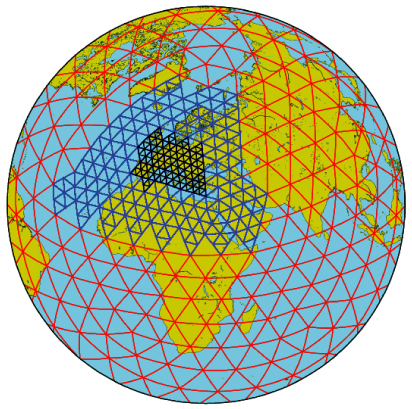
\includegraphics[height=200px]{bilder/gitternetz}
    \caption{Dreiecksgitter des ICON Wettermodells}
    \label{gitternetz}
  \end{center}
\end{figure}

Mit der Maschenweite bezeichnet man den horizontalen Abstand zwischen
zwei benachbarten Gitterpunkten. Je feiner das Gitter, bzw. je höher
die Auflösung des Modells ist, desto genauer kann die Erdoberfläche
und die darüber liegenden atmosphärischen Strukturen erfasst werden,
was sich auf die Genauigkeit der Wettervorhersage auswirkt. Die
benötigten Ressourcen zu Berechnung der Modellgleichungen steigt mit
der Anzahl der verwendeten Gitterpunkte.

Da eine sehr hohe Auflösungen selbst die Leistungsfähigkeit der
schnellsten Supercomputer übersteigt werden von den Wetterdiensten
meist verschiedene Modelle in unterschiedlichen Auflösungen
berechnet. Globale, den gesamten Globus umfassende Modelle werden mit
einer geringeren Auflösung als lokale, Länder oder Kontinente
abdeckende Modelle berechnet. Je weiter in die Zukunft prognostiziert
werden soll, desto mehr spielen aber wieder Wetterphänomene aus
Gebieten die nicht vom lokalen Modell abgedeckt werden eine Rolle. Für
Vorhersagen ab 5 Tagen in die Zukunft benötigen die lokalen Modelle
wiederum Informationen aus der gesamten Atmosphäre. Deshalb verwenden
die höher auflösenden lokalen Modelle oft Informationen als Randwerte
aus einem zuvor berechneten globalen Modell.

Die zeitliche Diskretisierung hingegen ist weniger problematisch. Die
meisten Modelle bieten mindestens Prognosen um 12 und 24 Uhr für
diejenigen Tage an, über die sich der Vorhersagezeitraum
erstreckt. Das \textit{Global Forecast System} Modell bietet
beispielsweise Vorhersagen im drei Stunden Intervall an, wobei das
lokale \textit{COSMO-DE} Modell mit einem 25 Sekunden Intervall
betrieben wird.

\subsubsection{Rechenaufwand heutiger Modelle}

In einer Präsentation
\footnote{\url{http://www.initiative-wissenschaftsjournalismus.de/fileadmin/Downloads/WissensWerte2008/B3_Majewski.pdf}}
aus dem November 2008 wurde der Rechenaufwand für die vom Deutschen
Wetterdienst betriebenen Modelle mit den dazugehörigen Kenngrößen
veröffentlicht. Damals wurden die Wettervorhersagen auf einem IBM
Power 5 System (p575) mit 52 Knoten, 416 Prozessoren und einer
Spitzenleistung von 3,1 Teraflop/s berechnet.

\begin{itemize}
\item Für Deutschland wird das \textit{COSMO-DE} Modell mit einer
  Maschenweite von 2,8 Kilometern betrieben und besteht aus ca. 10
  Millionen Gitterpunkten. Die Berechnung dauert 30 Minuten und
  liefert Vorhersagen in einem 25 Sekunden Intervall für einen
  21-stündigen Vorhersagezeitraum.
\item Das Europa umfassende Modell \textit{COSMO-EU} hat eine
  Maschenweite von 7 Kilometern, ca. 17 Millionen Gitterpunkten und
  wird mit einem Zeitintervall von 40 Sekunden erstellt. Die
  Berechnung einer 24-stündigen Vorhersage dauert 25 Minuten.
\item Das globale, die gesamte Welt umfassende \textit{GME} Modell hat
  eine Maschenweite von 40 Kilometern mit ca. 15 Millionen
  Gitterpunkten. Die Berechnung der 24 Stunden Vorhersage mit einem
  Zeitintervall von 133 Sekunden benötigt 15 Minuten.
\end{itemize}

Leider wurden während der Recherche keine genaueren Informationen
gefunden, wie sich die Berechnung der hier erwähnten Modelle auf dem
seit März 2009 beim Deutschen Wetterdienst in Betrieb genommenen
Vektorsupercomputer SX-9 der Firma NEC verhält. Die Spitzenleistung
dieses Systems beträgt momentan 4,5 Teraflop/s, die bis 2010 auf 11
Teraflop/s aufgestockt werden soll. Mit dieser neuen Anschaffung will
der Deutsche Wetterdienst unter anderem auch Wettervorhersagen mit
einer Auflösung von 2,8 Kilometern für Deutschlands Anrainerstaaten
berechnen.

\subsection{Geographische Breite und Länge}

Zur Festlegung von Punkten auf der Erde wird meist ein
Koordinatensystem genutzt, dessen Grundlage parallel zum Äquator
verlaufende Breitenkreise, und die beiden Pole verbindende
Längenhalbkreise sind. Der am Äquator angesiedelte Breitenkreis teilt
die Erde in die nördliche und die südliche Halbkugel. Sowohl auf dem
nördlichen als auch auf dem südlichen Teil verlaufen jeweils weitere
90 Kreise, den Äquator mit eingeschlossen also insgesamt 181
Breitenkreise. Die beiden Pole werden durch 360 nebeneinander liegende
Längenhalbkreise verbunden, von denen der durch die Sternwarte in
\textit{Greenwich} verlaufende Halbkreis als Nullmeridian bezeichnet
wird. Die Zählung fängt am Nullmeridian an, und geht jeweils um 180
Schritte in beide Richtungen. Nullpunkt des Koordinatensystems ist
derjenige Punkt, an dem der Nullmeridian den Äquator kreuzt. In
Abbildung \ref{koordinaten} ist der durch \textit{Greenwich} laufende
Nullmeridian und der 30 $^\circ$ nördlich verlaufende Breitenkreis zu
sehen.

\begin{figure}[h]
  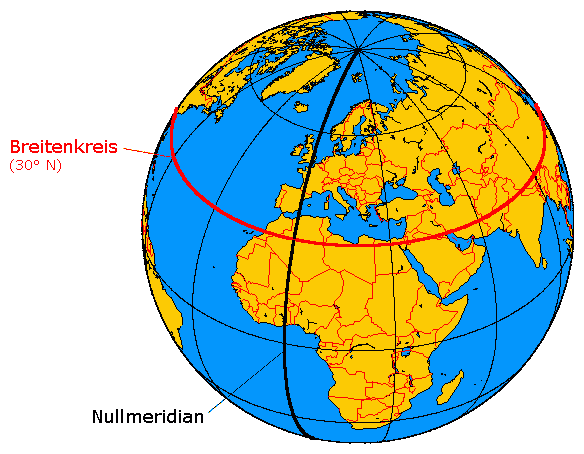
\includegraphics[width=310px]{bilder/koordinaten}
  \caption{Die in Breiten- und Längenkreise unterteilte Erdkugel}
  \label{koordinaten}
\end{figure}

Die Position eines Punktes auf der Erde wird durch seine geographische
Breite (\textit{Latitude}) und Länge (\textit{Longitude})
angegeben. Dies sind die in der Einheit Grad angegebenen, und vom
Nullpunkt aus gesehenen Abstände, der durch diesen Punkt verlaufenden
Breiten- und Längenkreise. Die Position von \textit{Greenwich} ist
beispielsweise durch die Angabe \textit{51.479 $^\circ$ N, 0.0
  $^\circ$ E} festgelegt.


\subsection{Angaben zur Modellauflösung}
Das \textit{Global Forecast System} und das \textit{Wave Watch III}
Modell beziehen sich ebenfalls auf dieses Koordinatensystem, und deren
Gitterauflösung wird der Einheit Grad angegeben. Da die meisten
Menschen aber bei Distanzangaben in einer Längeneinheit denken an die
sie gewöhnt sind und unter der sie sich auch etwas vorstellen können,
stellt sich die Frage wieviel Kilometer bzw. Meilen der Abstand
zwischen zwei Knotenpunkten des Gitternetzes beträgt.

Aufgrund der elipsoiden Gestalt der Erdkugel kann hierzu jedoch keine
allgemeingültige Aussage getroffen werden, da dies von der jeweils
betrachteten Region auf der Erdkugel und dem verwendeten
Referenzellipsoiden abhängig ist. Ein Breitengrad (\textit{Latitude})
entspricht durchschnittlich etwa 111 Kilometern und ist weitestgehend
konstant. Der Abstand zwischen den Längengraden (\textit{Longitude})
variiert allerdings erheblich. Am Äquator beträgt dieser Abstand
ebenfalls ungefähr 111 Kilometer, konvergiert aber an den Polen in
Richtung Null. Die hier teilweise in Kilometern angegebenen
Gitterauflösungen sind demnach nur als grobe Richtwerte zur besseren
Einschätzung der Gitterauflösung zu verstehen und beziehen sich auf
die Regionen um den Äquator. Praktische Zusammenfassungen mit
entsprechende Formeln zur Berechnung von Problemen aus dem
geographischen Bereich sind unter \cite{aviation} und
\cite{movable_type_scripts} zu finden.

\subsection{Global Forecast System}

Das \textit{Global Forecast System} ist ein globales numerisches
Wettermodell das vom \textit{National Weather Service} betrieben wird
und den gesamten Erdball abdeckt. Da die Ergebnisse der
Modellberechnung über das Internet
\footnote{\url{http://nomad5.ncep.noaa.gov/pub/gfs}} erhältlich sind
und von jedermann verwendet werden dürfen erfreut es sich einer großen
Beliebtheit. Das Modell liefert Vorhersagen bis zu 384 Stunden (16
Tage) in die Zukunft und wird mit variierenden Auflösungen viermal
täglich berechnet, jeweils um 0h, 6h, 12h und 18h koordinierter
Weltzeit (\textit{UTC}). Die ersten 180 Stunden werden mit einer
Maschenweite von ca. 40 Kilometern und einem Intervall von 3 Stunden
berechnet, die restlichen Stunden im 12 Stunden Intervall und einer
Auflösung von ca. 80 Kilometern. Vertikal wird die Atmosphäre bei
beiden Auflösungen in 64 unterschiedliche Luftschichten aufgeteilt.

Das Modell berechnet eine Vielzahl von physikalischen Größen, von
denen hier hauptsächlich die Temperatur, die Gesamtbewölkung und das
Niederschlagswasser von Bedeutung sind. Da weithin Einverständnis
darüber herrscht, dass Vorhersagen über 180 Stunden hinaus sehr
ungenau sind verwenden die hier entwickelten \textit{ETL} Prozessen
nur die ersten 180 Stunden in der hohen Auflösung.

\subsection{Wave Watch III}

Um für mehr Sicherheit auf hoher See und an Küstenregionen zu sorgen
betreibt der \textit{National Weather Service} das \textit{Wave Watch
  III} Wettermodell um Wellen vorherzusagen. Es liefert ausschließlich
Informationen über diejenigen Wellen, die durch den direkten Einfluss
von Winden entstehen. Wellen die durch andere Ereignisse wie
z.B. Gewitter, Gezeiten oder Tsunamis verursacht werden, sind in
diesem Modell nicht berücksichtigt. Da sich Wellen viel zu sehr
voneinander unterscheiden, werden nicht Vorhersagen für einzelne
Wellen getroffen, sondern über die Statistik mehrerer Wellen. Das
Modell liefert sowohl Informationen über die Wellenhöhe, Wellenperiode
und Wellenrichtung als auch über die Windstärke und die Windrichtung
an einem bestimmten Ort zu einer bestimmten Zeit.

Das Modell wird wie das \textit{Global Forecast System} viermal
täglich neu berechnet, liefert Vorhersagen im 3 Stunden Intervall für
180 Stunden in die Zukunft und die Ergebnisse sind ebenfalls frei
erhältlich
\footnote{\url{http://polar.ncep.noaa.gov/waves/index2.shtml}}. Das
globale Modell wird mit einer Maschenweite von ca. 80 Kilometern
berechnet, die lokalen Modelle mit einer Maschenweite von bis zu 20
Kilometern. Die hier entwickelten \textit{ETL} Prozesse verarbeiten
bisher nur die Daten des globalen Modells.

\section{Das Gridded Binary Datenformat}

Die Abkürzung \textit{Grib} \nomenclature{GRIB}{Gridded Binary} steht
für \textit{GRIdded Binary} und ist ein bitorientiertes Datenformat
zum Speichern und Übertragen von Wetterdaten. Das Format wurde von der
\textit{Kommission für Basissysteme} (\textit{CBS})
\nomenclature{CBS}{Commission for Basic Systems} der
\textit{Weltorganisation für Meteorologie} (\textit{WMO})
\nomenclature{WMO}{World Meteorological Organization} standardisiert
\footnote{\url{http://www.wmo.int/pages/prog/www/WMOCodes/Guides/GRIB/GRIB1-Contents.html}}
und wird von vielen Wetterorganisationen dazu verwendet die Ergebnisse
ihrer Modellberechnungen kompakt und plattformunabhängig zu
speichern. Insgesamt wurden drei verschiedenen Versionen spezifiziert,
von denen sich die Versionen 1 und 2 etabliert haben. Die mit der
Nummer 0 bezeichnete Version wird als veraltet angesehen und befindet
sich bei den meisten Wetterorganisationen nicht mehr im operativen
Einsatz.

\subsection{Struktur von Grib Dateien}

Eine \textit{Grib} Datei besteht aus eigenständigen, sich selbst
beschreibenden Datensätzen, den sogenannten \textit{Grib}
Nachrichten. Eine Nachricht enthält dabei alle Daten eines bestimmten
Vorhersageelements, für eine auf ein Gitternetz diskretisierte
geographische Region zu einem bestimmten Zeitpunkt. Beispielsweise die
Temperaturen um 12 Uhr mittags für Europa aus dem \textit{Global
  Forecast System}, oder die signifikanten Wellenhöhen des
\textit{Wave Watch III} Modells um 9 Uhr morgens für die gesamte
Erdkugel.

Eine \textit{Grib} Nachricht besteht wiederum aus mehreren Sektionen,
die deren Inhalt genauer beschreiben und in Tabelle \ref{tab:grib}
aufgelistet sind. Die Sektionen enthalten neben den eigentlichen Daten
u.a. Informationen über die Dimension und Auflösung des verwendeten
Gitternetzes, die Herkunft der Daten, die Art des verwendeten
Komprimierungsverfahrens und die physikalische Einheit in der die
Daten gespeichert sind.

\begin{table*}
  \centering
  {\sf
    \footnotesize
    \begin{longtable}{@{}lp{10cm}@{}}

      \toprule
      \textbf{Name der Sektion} & \textbf{Verwendungszweck} \\

      \midrule

      Indicator & Die Zeichenkette ''GRIB'', Versionsnummer, Länge der gesamten Nachricht \\

      Identification & Charakteristiken die auf alle Daten zutreffen, u.a. Herkunft der Daten, Referenzzeit und Typ des Produkts \\

      Local Use (optional) & Abschnitt für beliebige zusätzliche Informationen \\

      Grid Definition &  Definition des Gitternetzes, u.a. die Dimension, die Anzahl der Datenpunkte und die verwendete Koordinatenprojektion \\

      Product Definition &  Beschreibung der Daten. \\

      Data Representation &  Beschreibung wie die Daten repräsentiert werden. Art der Komprimierung \\

      Bitmap & Eine Bitmap, welche die Anwesenheit bzw. Abwesenheit von Datenpunkten in der nächsten Sektion signalisiert \\

      Data &  Die komprimierten Daten. Für jeden in der Bitmap existierenden Gitterpunkt ein Wert. \\

      End & Die Zeichenkette ''7777'' markiert das Ende der Nachricht \\

      \bottomrule

    \end{longtable}
  }

  \caption{Die aufeinander folgenden Sektionen einer \textit{Grib2} Nachricht}
  \label{tab:grib}

\end{table*}

\textit{Grib} Nachrichten können beliebig oft aneinandergereiht
werden, was eine individuelle Komposition von beliebigen Nachrichten
in einer Datei erlaubt. Dies wird in Abschnitt \ref{subsec:download}
ausgenutzt um nur ausgewählte Nachrichten aus einer größeren
\textit{Grib} Datei zu beziehen.

\subsection{Programme zum Verarbeiten von Grib Dateien}
\label{grib-reader}

Zum Verarbeiten und Lesen von \textit{Grib} Dateien werden spezielle
Programme eingesetzt. Werkzeugen für die Kommandozeile, C-Bibliotheken
und Programmen zur Visualisierung der \textit{Grib} Daten sind für
verschiedene Plattformen und Programmiersprachen erhältlich. Eine
Übersicht gängiger Software ist bei \textit{Wikipedia}
zusammengestellt.
\footnote{\url{http://en.wikipedia.org/wiki/GRIB\#Applications}} Zur
Weiterverarbeitung sind insbesondere die Kommandozeilenprogramme
\texttt{wgrib} und \texttt{degrib} zu empfehlen, da sie als typische
\textit{UNIX} Filter konzipiert sind und in Kombination mit
\textit{UNIX} Standardwerkzeugen wie z.B. \texttt{cat}, \texttt{curl}
oder \texttt{dd} flexibel eingesetzt werden können. Das Programm
\texttt{degrib} bietet die Möglichkeit einen Index für eine
\textit{Grib} Datei zu generieren, mit dessen Hilfe ein wahlfreier
Zugriff nach geographischen Positionen ermöglicht wird und die
Zugriffszeiten erheblich beschleunigt.

\subsection{Inventar einer Grib Datei}

Die beiden Kommandozeilenprogramme \texttt{degrib} und \texttt{wgrib}
können dazu verwendet werden Inventare von \textit{Grib} Datei zu
erstellen. Ein Inventar ist eine Art Inhaltsverzeichnis und liefert
Informationen über die in der Datei enthaltenen Nachrichten. Da
\textit{Grib} Dateien oft mehrere Megabyte groß sind, stellen viele
Wetterorganisationen aus praktischen Gründen zusätzlich die Inventare
zur Verfügung. Ein Inventar ist zur Verarbeitung einer \textit{Grib}
Datei zwar nicht zwingend erforderlich, vereinfacht aber den Umgang,
da nicht immer die kompletten \textit{Grib} Dateien übertragen werden
müssen, sondern nur die sehr viel kleineren Inventare. In Abbildung
\ref{abbildung:inventar} ist der Ausschnitt eines Inventars von einer
\textit{Grib} Datei des \textit{Global Forecast System} zu sehen. Pro
Nachricht ist in diesem Inventar eine Zeile enthalten, die unter
anderem Informationen über die Nummer der Nachricht, deren Position in
Bytes und den Zeitpunkt als auch das Element der Vorhersage, bzw. der
Analyse liefert.

\begin{figure}[h]
  \begin{Verbatim}[frame=lines,framerule=0.5pt,framesep=3mm]
    1:0:d=2009081812:HGT:10 mb:anl:NAve=0
    2:519924:d=2009081812:TMP:10 mb:anl:NAve=0
    3:812418:d=2009081812:UGRD:10 mb:anl:NAve=0
    ...
    568:211123530:d=2009081812:VWSH:-1500 pv units:anl:NAve=0
  \end{Verbatim}
  \caption{Inventar einer \textit{Grib} Datei des \textit{Global
      Forecast System} }
  \label{abbildung:inventar}
\end{figure}

Die zweite Zeile aus Abbildung \ref{abbildung:inventar} gibt zum
Beispiel Auskunft darüber, dass die Nachricht mit der Nummer 2 in der
\textit{Grib} Datei an der Position 519.924 (Byte) zu finden ist, die
Werte der Nachricht für den 18. August 2009 um 12 Uhr gelten, und das
Element die Temperatur (TMP) auf einer Höhe von 10 Hektopascal (10 mb)
darstellt. Zudem handelt es sich bei den Werten nicht um eine
Vorhersage (fcst), sondern um eine Analyse (anl) für die kein
durchschnittlicher Wert (NAve=0) vorhanden ist.

\section{Extraktion aus dem Quellsystem}

Die Aufgabe der hier entwickelten Extraktionsprozesse besteht darin,
die benötigten Daten des \textit{Wave Watch III} Models und des
\textit{Global Forecast Systems} herunterzuladen, und diese in einer
einheitlichen Struktur für die Weiterverarbeitung im lokalen
Dateisystem zu hinterlegen. Da insbesondere das Datenvolumen des
\textit{Global Forecast System} in seiner höchsten Auflösung sehr
umfangreich ist (ca. 13 GB), wird ein Verfahren angewendet, um nur
ausgewählte Daten beider Modelle zu beziehen. In diesem Abschnitt wird
zuerst die Struktur des Quellsystems analysiert, dann das erwähnte
Verfahren zum Download der reduzierten Daten vorgestellt, und
anschließend eine Aussage über die Performanz der Extraktionsprozesse
getroffen.

\subsection{Analyse der Quellsystems}

Sowohl das \textit{Global Forecast System} als auch das \textit{Wave
  Watch III} Modell werden viermal täglich, jeweils um 0h, 6h, 12h und
18h koordinierter Weltzeit berechnet. Danach werden die Ergebnisse in
\textit{Grib} Dateien auf mehreren, teilweise von Unterorganisationen
der \textit{National Oceanic and Atmospheric Administration}
betriebenen Servern veröffentlicht, die verschiedensten Anforderungen
gerecht werden. Auf einigen Server sind nur die aktuellen Ergebnisse
verfügbar, andere wiederum dienen zur Archivierung und bieten eine
Historie über mehrere Jahre hinweg.

Die Ergebnisse der Modellberechnung werden in einem, meist nach Datum
und Uhrzeit strukturierten Dateisystem hinterlegt, das per
\textit{FTP} oder \textit{HTTP} exportiert wird. Die Struktur und
Benennung der Verzeichnisse und Dateien variiert dabei zwischen den
Servern, ist aber innerhalb eines Servers konsistent und folgt einem
vorhersehbaren Muster. Die \textit{URI}s der benötigten Daten können
so für einem bestimmten Server im voraus konstruiert werden und deren
Existenz mit einem der unterstützten Protokolle überprüft
werden. Dieses Verfahren kann als Anwendungsbeispiel zur
Identifizierung von Ressourcen durch vorhersehbare \textit{URI}s
angesehen werden, und ist einer der in Abschnitt
\ref{paragraph:identifizierung} beschriebenen Vorschläge der
\textit{Ressource Oriented Architecture}.

\subsubsection{Datenorganisation des Global Forecast System}

Aktuelle Daten des \textit{Global Forecast System} können in
verschiedenen Auflösung von den Servern des \textit{National Oceanic
  And Atmospheric Administration Operational Model Archive and
  Distribution System (NOMADS)} \nomenclature{NOMADS}{NOAA Operational
  Model Archive and Distribution System}
\footnote{\url{http://nomads.ncdc.noaa.gov}} bezogen werden. In
Tabelle \ref{tab:gfs_auflösungen} sind die Dateigrößen und
Bezugsquellen der \textit{Grib} Dateien in den verschiedenen
Auflösungen dargestellt. Die Dateigröße bezieht sich dabei immer auf
eine einzelne \textit{Grib} Datei, die alle Vorhersageelemente des
\textit{GFS} für einen bestimmten Zeitpunkt in der Zukunft enthält.

\begin{table*}[h]
  \centering
  {\sf
    \footnotesize
    \begin{longtable}{@{}ccl}

      \toprule
      \textbf{Auflösung} & \textbf{Dateigrößen} & \textbf{URI der Bezugsquelle} \\

      \midrule

      2$^{\circ}$ x 5$^{\circ}$ & 4 Mb - 4.8 Mb & \url{http://nomad5.ncep.noaa.gov/pub/gfs2p5} \\
      1$^{\circ}$ x 1$^{\circ}$ & 25 Mb - 29 Mb & \url{http://nomad5.ncep.noaa.gov/pub/gfs} \\
      0.5$^{\circ}$ x 0.5$^{\circ}$ & 200 Mb - 215 Mb & \url{http://nomad5.ncep.noaa.gov/pub/gfs_master} \\

      \bottomrule

    \end{longtable}
  }

  \caption{Dateigrößen der verschiedenen Auflösungen des GFS}
  \label{tab:gfs_auflösungen}

\end{table*}

Die in dieser Arbeit entwickelten \textit{ETL} Prozesse arbeiten alle
mit den \textit{Grib} Dateien der höchsten Auflösung
(0.5$^{\circ}$ x 0.5$^{\circ}$). Unter der \textit{URI}
\url{http://nomad5.ncep.noaa.gov/pub/gfs_master/} sind Verzeichnisse
zu finden, die nach dem Muster \texttt{gfs\textbf{YYYYMMDD}} benannt
sind. Dabei steht \texttt{YYYY} für das Jahr, \texttt{MM} für den
Monat und \texttt{DD} für den Tag, an dem ein Modell berechnet
wurde. Beispielsweise waren die \textit{Grib} Dateien aller
Modellberechnungen, die am 16. August 2009 durchgeführt wurden unter
der \textit{URI}
\url{http://nomad5.ncep.noaa.gov/pub/gfs_master/gfs20090816/}
aufgelistet.  \footnote{Der Server \texttt{nomad5.ncep.noaa.gov}
  verwaltet keine historischen Daten, d.h. wenn dieses Dokument
  gelesen wird sind höchstwahrscheinlich keine Daten mehr vorhanden.}

In den nach Tagen geordneten Verzeichnissen befinden sich
\textit{Grib} Dateien die nach dem Muster
\texttt{gfs.t\textbf{XX}z.master.grbf\textbf{YY}} benannt sind. Die Zeichen
\texttt{XX} stehen dabei für den Zeitpunkt der Modellberechnung (00,
06, 12 oder 18), und die Zeichen \texttt{YY} für die Stunde der
Vorhersage in der Zukunft (00-180 im 3 Stunden Intervall). Die
Vorhersagedaten des \textit{GFS} für den 16. August 2009 um 18 Uhr
abends, die am selben Tag um 6 Uhr morgens berechnet wurden, waren
somit in der \textit{Grib} Datei mit der \textit{URI}
\url{http://nomad5.ncep.noaa.gov/pub/gfs_master/gfs20090816/gfs.t06z.master.grbf12}
zu finden.

Eine \textit{Grib} Datei des \textit{Global Forecast System} enthält
für einen bestimmten Zeitpunkt 63 verschiedene Vorhersageelemente und
ist zwischen 200 und 215 Megabyte groß. Die Größe aller \textit{Grib}
Daten für einen Vorhersagezeitraum von 180 Stunden (und für den
Berechnungszeitpunkt selbst) mit einem 3-stündigen Intervall beträgt
somit $(180h / 3h + 1) * 215 Mb = 13115 Mb$. Da aber nur sehr wenige
Vorhersageelemente der \textit{Grib} Dateien benötigt werden, wird in
Abschnitt \ref{subsec:download} ein Verfahren vorgestellt, um nur die
benötigten Elemente zu übertragen, und somit das Datenvolumen zu
reduzieren.

\subsubsection{Datenorganisation des Wave Watch III Models}
Die Daten des \textit{Wave Watch III} Modells sind ähnlich
strukturiert wie die des \textit{Global Forecast System}, und werden
in einer Auflösung von 1.25$^{\circ}$ x 1$^{\circ}$ ebenfalls auf den
\textit{NOMADS} Servern veröffentlicht. Die \textit{Grib} Dateien
werden in Verzeichnissen hinterlegt, die nach dem Muster
\texttt{nww3\textbf{YYYYMMDD}} benannt, und unter der \textit{URI}
\url{http://nomad5.ncep.noaa.gov/pub/waves/nww3} angeordnet sind. Auch
hier ist das Datum der Modellberechnung im Verzeichnisnamen
kodiert. Das \textit{Wave Watch III} Modell hat im Vergleich zum
\textit{Global Forecast System} viel weniger Elemente, weshalb die
kompletten Daten für eine 180-stündige Vorhersage in einer einzigen
Datei gespeichert werden. Diese ist nach dem Muster
\texttt{nww3.t\textbf{XX}z.grib} benannt, wobei \texttt{XX} hier
ebenfalls für den Zeitpunkt der Modellberechnung (00, 06, 12 oder 18)
steht. Die Ergebnisse des \textit{Wave Watch III} Modells, das z.B. am
16. August 2009 um 18 Uhr berechnet wurde, konnten unter der
\textit{URI}
\url{http://nomad5.ncep.noaa.gov/pub/waves/nww3/nww320090816/nww3.t18z.grib}
bezogen werden.

Eine \textit{Grib} Datei des \textit{Wave Watch III} Models mit 11
verschiedenen Elementen ist bei einer Auflösung von
1.25$^{\circ}$ x 1$^{\circ}$ ca. 32 Megabyte groß und enthält
Vorhersagedaten für 180 Stunden in die Zukunft.

\subsection{Download einzelner Grib Nachrichten}
\label{subsec:download}

Die eben beschriebenen Vorhersagemodelle bieten sehr viel mehr
Informationen zum Download an, als von der hier entwickelten
Anwendungen überhaupt benötigt wird. Vom \textit{Global Forecast
  System} werden im Moment lediglich 4 der 63 verschiedenen
Vorhersagelemente, und vom \textit{Wave Watch III} Modell 7 von 11
Elementen verwendet. Um nicht unnötig Bandbreite zu verschwenden, und
den Extraktionsprozess zu beschleunigen, wird hier ein Verfahren
verwendet, das in dem Dokument \textit{Fast Downloading of Grib Files}
\footnote{\url{http://www.cpc.noaa.gov/products/wesley/fast_downloading_grib.html}}
beschrieben ist. Ziel ist es nur die gewünschten Nachrichten einer
\textit{Grib} Datei herunterzuladen. Voraussetzung dafür ist, dass die
Dateien von einem Server bezogen werden, der das HTTP/1.1 Protokoll
unterstützt, und die Inhaltsverzeichnisse der Dateien zu Verfügung
stehen. Das Verfahren besteht aus den folgende drei Schritten.

\begin{enumerate}
\item Download des Inhaltsverzeichnisses der entsprechenden Datei
\item Berechnung der Start- und Endpositionen aller relevanten Nachrichten
\item Download der entsprechenden Nachricht (\textit{HTTP Range Header})
\end{enumerate}

Im ersten Schritt wird das Inhaltsverzeichnis der entsprechenden
\textit{Grib} Datei heruntergeladen. Die Inhaltsverzeichnisse auf den
\textit{NOMADS} Servern sind mit dem \textit{wgrib} Programm erstellt,
und deren \textit{URI} lässt sich durch das Anhängen der Endung
''.inv'', an die \textit{URI} der \textit{Grib} Datei konstruieren.

Anschließend wird im zweiten Schritt in Zweierpaaren über die Zeilen
des Inhaltsverzeichnisses iteriert. Dabei wird die Startposition jeder
Nachricht extrahiert, und die dazugehörige Endposition berechnet. Die
Startposition steht dabei an zweiter Stelle jeder Zeile, und die
Endposition berechnet sich aus der Startposition der nächsten
Nachricht, von der ein Byte subtrahiert wird. Ein Sonderfall ist die
letzte Nachricht des Inhaltsverzeichnisses. Für diese Nachricht kann
die Endposition nicht berechnet werden, da keine Information über die
gesamte Länge der \textit{Grib} im Inhaltsverzeichnis vorhanden
ist. Tabelle \ref{tab:inhaltsverzeichnis_mit_positionen} zeigt das
Resultat dieser Berechnung, angewendet auf das Inhaltsverzeichnis aus
Abbildung \ref{abbildung:inventar}.

\begin{table*}[h]
  \centering
  {\sf
    \footnotesize
    \begin{longtable}{@{}ccccc}
      \toprule
      \textbf{Nachricht} & \textbf{Startposition} & \textbf{Endposition} & \textbf{Referenzzeit} & \textbf{Element} \\
      \midrule
      1 & 0 & 519.923 & 2009-08-18 12:00 & HGT \\
      2 & 519.924 & 812.417 & 2009-08-18 12:00 & TMP \\
      3 & 812.418 & ... & 2009-08-18 12:00 & UGRD \\
      ... & ... & ... & ... & ... \\
      568 & 211.123.530 & - & 2009-08-18 12:00 & HGT \\
      \bottomrule
    \end{longtable}
  }

  \caption{Berechnete Positionen aus einem Inhaltsverzeichnis}
  \label{tab:inhaltsverzeichnis_mit_positionen}

\end{table*}

Im dritten Schritt werden schließlich nur die ausgewählten Nachrichten
unter Verwendung des \textit{HTTP/1.1} Protokolls
heruntergeladen. Dabei wird pro Nachricht eine Anfrage an den Server
gesendet, in der die Start- und Endposition im \textit{Range} Feld des
\textit{HTTP} Headers eingetragen wird. Um beispielsweise nur die
zweite Nachricht aus Tabelle
\ref{tab:inhaltsverzeichnis_mit_positionen} herunterzuladen, wird das
\textit{Range} Feld auf ''bytes=519924-812417'' gesetzt. Der im
zweiten Schritt erwähnte Sonderfall, bei dem die Endposition für die
letzte Nachricht nicht bekannt ist, wird dadurch abgedeckt, dass die
Endposition im \textit{Range} Header einfach weggelassen wird. Dies
ist trotz der fehlenden Endposition eine gültige \textit{Range} Angabe
und veranlasst den Server dazu den Rest der Datei ab der gegebenen
Startposition zu senden.

\subsection{Beschreibung der Extraktionsprozesse}

Ziel der Extraktion ist es alle relevanten \textit{Grib} Nachrichten
der beiden Modelle in einer einheitlichen Struktur im lokalen
Dateisystem zu hinterlegen. Pro Element soll dabei eine Datei erstellt
werden, die alle Nachrichten des entsprechenden Elements für die
verschiedenen Zeitpunkte der Vorhersage enthält. Beim Download der
\textit{Grib} Dateien von den \textit{NOMADS} Servern werden zwei
verschiedene Strategien angewendet, die im Folgenden beschrieben
werden. Dies ist auf die unterschiedliche Datenorganisation der beiden
Vorhersagemodelle auf der Serverseite zurückzuführen.

Die Performanz der Extraktionsprozesse hängt hauptsächlich von der
Geschwindigkeit ab, mit der die \textit{Grib} Daten heruntergeladen
werden. Zu verschiedenen Zeiten durchgeführte Benchmark Tests ergaben
eine eher mäßige durchschnittliche Übertragungsgeschwindigkeit von
186.30 KB/s. Dies liegt vermutlich an der hohen Auslastung der
\textit{NOMADS} Server, auf die keinen Einfluss genommen werden
kann. Um eine besser und einen längerfristigen Zeitraum abdeckende
Aussage zu machen, wurden die Log Dateien des Extraktionsprozesse aus
einem Zeitraum von einer Woche ausgewertet und die Ergebnisse
zusammengefasst.

\subsubsection{Downloadstrategie für das Wave Watch III Model}
Alle Daten des \textit{Wave Watch III} Modells sind auf Serverseite in
einer \textit{Grib} Datei gespeichert. Der Extraktionsprozess für
dieses Modell lädt zunächst das Inhaltsverzeichnis dieser Datei, um
die Start- und Endpositionen der gewünschten Elemente zu
berechnen. Anschließend wird pro Element eine \textit{HTTP-Range}
Anfrage an den Server gesendet, und die in der Antwort enthaltene
\textit{Grib} Nachricht in einer Datei im lokalen Dateisystem
gespeichert.

\begin{table*}[h]
  \centering
  {\sf
    \footnotesize
    \begin{longtable}{@{}clccc}
      \toprule
      \textbf{Element} & \textbf{Beschreibung} & \textbf{Größe (Element)} & \textbf{Zeit (Element)}  \\
      \midrule
      HTSGW & Wellenhöhe & 2.5 MB & 27.12 s \\
      PERPW & Periode des Wellenkamms & 2.7 MB & 30.12 s \\
      DIRPW & Richtung des Wellenkamms & 3.5 MB & 35.90 s \\
      WVPER & Wellenperiode & 2.5 MB & 25.79 s \\
      WVDIR & Wellenrichtung & 3.5 MB & 35.83 s \\
      WIND  & Windstärke & 2.9 MB & 34.36 s \\
      WDIR  & Windrichtung & 3.8 MB & 38.99 s \\
      \midrule
      Gesamt: & & 21.4 MB & 3.80 m \\
      \bottomrule
    \end{longtable}
  }
  \caption{Messung der Downloadzeiten des \textit{Wave Watch III} Modells}
  \label{tab:download_messung_ww3}
\end{table*}

Insgesamt werden bei einem Durchlauf 8 Anfragen an den Server
gesendet, eine für das Inhaltsverzeichnis und 7 für die \textit{Grib}
Nachrichten der entsprechenden Elemente. In Tabelle
\ref{tab:download_messung_ww3} sind die durchschnittlichen
Downloadzeiten für die einzelnen Elemente des \textit{Wave Watch III}
Modells aufgeführt. Der Extraktionsprozess dauert durchschnittlich 3.8
Minuten und überträgt \textit{Grib} Daten mit einem Volumen von 21.4
MB.

\subsubsection{Downloadstrategie für das Global Forecast System}

Der Downloadvorgang für das \textit{Global Forecast System} erfordert
wesentlich mehr Anfragen als der des \textit{Wave Watch III} Modells,
da die Daten auf Serverseite in mehreren Dateien gespeichert sind. Für
jeden Zeitpunkt der Vorhersage existiert auf dem Server eine Datei, in
der die Daten aller Modellelemente für den entsprechenden Zeitpunkt
enthalten sind. Dies sind bei einem Vorhersagezeitraum von 180 Stunden
im 3-stündigen Intervall 61 Dateien, $180h / 3h = 60$ für den
Vorhersagezeitraum, und eine weitere für den Zeitpunkt der Analyse.

Um alle \textit{Grib} Nachrichten für ein ausgewähltes Element
herunterzuladen, müssen zunächst die 61 Inhaltsverzeichnisse aller
\textit{Grib} Dateien angefordert werden, damit die Start- und
Endpositionen des Elements berechnet werden können. Anschließend
können die eigentlichen Daten des Elements mit \textit{Http-Range}
Anfragen aus den 61 \textit{Grib} Dateien heruntergeladen werden. Die
einzelnen \textit{Grib} Nachrichten aus den Dateien werden dann pro
Element in einer Datei zusammengefasst. Dies kann Dank des
selbstbeschreibendem Format der einzelnen \textit{Grib} Nachrichten
mit Standard Unix Kommandos bewerkstelligt werden, beispielsweise mit
\textit{cat TMP.00h.grib TMP.03h.grib ... TMP.180h.grib >
  TMP.0h-180h.grib}. Bis auf das Anfordern der Inhaltsverzeichnisse
muss dieser Vorgang für alle gewünschten Elemente wiederholt werden.

\begin{table*}[h]
  \centering
  {\sf
    \footnotesize
    \begin{longtable}{@{}ccccc}
      \toprule
      \textbf{Element} & \textbf{Größe (Nachricht)} & \textbf{Zeit (Nachricht)} & \textbf{Größe (Element)} & \textbf{Zeit (Element)} \\
      \midrule
      TMP   & 317.4 KB & 4.17 s & 18.90 MB & 4.24 m \\
      TCDC  & 222.2 KB & 2.62 s & 13.23 MB & 2.66 m \\
      PWAT  & 317.4 KB & 3.63 s & 18.90 MB & 3.69 m \\
      WEASD & 285.6 KB & 3.27 s & 17.01 MB & 3.33 m \\
      \midrule
      Gesamt: & 1.12 MB  & 13.69 s & 68.04 MB & 13.92 m \\
      \bottomrule
    \end{longtable}
  }
  \caption{Messung der Downloadzeiten des \textit{Global Forecast System}}
  \label{tab:download_messung_gfs}
\end{table*}

Insgesamt sind $ 61 * (N+1) $ Anfragen nötig, 61 für die
Inhaltsverzeichnisse, und pro Element weitere \textit{61} Anfragen für
die einzelnen Grib Nachrichten. Der Extraktionsprozess für das
\textit{Global Forecast System} sendet somit für die zurzeit 4
verwendeten Elemente $ 61 * (4+1) = 305$ Anfragen.

Tabelle \ref{tab:download_messung_gfs} zeigt im linken Teil die Größe
einer einzelnen Nachrichten und die Zeit die benötigt wird um diese
herunterzuladen. Im rechten Teil ist die Zusammenfassung dieser Werte
für das jeweilige Element zu sehen. Des Extraktionsprozess für das
\textit{Global Forecast System} überträgt insgesamt 68.04 MB und
benötigt durchschnittlich ca. 14 Minuten.

\subsubsection{Lokales Grib Repository}
Nachdem der Extraktionsvorgang erfolgreich abgeschlossen wurde liegen
die \textit{Grib} Daten beider Modelle in einem \textit{Repository}
auf dem lokalen Dateisystem. Das \textit{Repository} ist dabei nach
dem Namen des Modells, dem Zeitpunkt an dem das Modell erstellt wurde
und dem Element der Vorhersage organisiert. Diese in Tabelle
\ref{tab:repository} zu sehende Struktur bietet den anschließenden
Transformationsprozessen einen einheitlichen Zugriff auf die Elemente
der Modelle.

\begin{table*}[h]
  \centering
  {\sf
    \footnotesize
    \begin{longtable}{@{}cccl}
      \toprule
      \textbf{Größe} & \textbf{Datum} & \textbf{Uhrzeit} & \textbf{Pfad im Repository} \\
      \midrule
      19 MB & 2009-08-18 & 16:19 & forecasts/gfs/20090818/t06z.PWAT.grib \\
      14 MB & 2009-08-18 & 16:13 & forecasts/gfs/20090818/t06z.TCDC.grib \\
      19 MB & 2009-08-18 & 16:09 & forecasts/gfs/20090818/t06z.TMP.grib \\
      18 MB & 2009-08-18 & 16:24 & forecasts/gfs/20090818/t06z.WEASD.grib \\
      \midrule
      3.5 MB & 2009-08-18 & 15:58 & forecasts/nww3/20090818/t06z.DIRPW.grib \\
      2.4 MB & 2009-08-18 & 15:57 & forecasts/nww3/20090818/t06z.HTSGW.grib \\
      2.8 MB & 2009-08-18 & 15:57 & forecasts/nww3/20090818/t06z.PERPW.grib \\
      3.9 MB & 2009-08-18 & 16:02 & forecasts/nww3/20090818/t06z.WDIR.grib \\
      3.0 MB & 2009-08-18 & 16:01 & forecasts/nww3/20090818/t06z.WIND.grib \\
      3.5 MB & 2009-08-18 & 16:00 & forecasts/nww3/20090818/t06z.WVDIR.grib \\
      2.5 MB & 2009-08-18 & 15:59 & forecasts/nww3/20090818/t06z.WVPER.grib \\
      \bottomrule
    \end{longtable}
  }
  \caption{Verzeichnisstruktur der Grib Daten im lokalen Repository}
  \label{tab:repository}
\end{table*}

\subsubsection{Aktualisierung der Daten durch Polling}
Zwar werden beide Modelle viermal täglich zu fixen Zeitpunkten
berechnet, wann genau die \textit{Grib} Dateien auf den
\textit{NOMADS} Servern allerdings zur Verfügung stehen variiert
allerdings etwas. Deshalb wird die Verfügbarkeit neuer Daten mittels
\textit{Polling} überprüft. Die durch \textit{Cronjob} gesteuerten
Prozesse überprüfen in einem bestimmten Intervall die Existenz der
Quelldaten, und starten den Extraktionsvorgang erst, wenn neue, noch
nicht integrierte Daten zur Verfügung stehen.

\subsubsection{Beurteilung der Extraktionsprozesse}
Trotz der eher mäßigen Übertragungsgeschwindigkeit kann die Performanz
der beiden Extraktionsprozesse als zufriedenstellend eingestuft
werden. Kritisch wird es, wenn die beanspruchte Zeit zum Extrahieren
der Daten sich dem 4-stündigen Intervall der Modellberechnung
nähert. Von dieser Grenze sind die beiden Prozesse jedoch noch
ausreichend weit entfernt. Da es den Anschein macht, dass die
Übertragungsgeschwindigkeit von den \textit{NOMADS} Servern pro
Verbindung reguliert wird, könnte versucht werden mehrere Anfragen
gleichzeitig zu stellen, um die Daten parallel herunterzuladen und
somit die Performanz zu verbessern.

\section{Transformation der Daten}
Nachdem der Extraktionsvorgang erfolgreich abgeschlossen wurde, und
die Daten beider Modelle im lokalen \textit{Repository} vorliegen,
startet die Transformationsphase. In dieser Phase wird die bisher noch
den gesamten Globus umfassende Datenmenge auf die in der Datenbank
enthaltenen \textit{Spots} reduziert. Alle relevanten Datensätze
werden dabei in einer \textit{CSV} \nomenclature{CSV}{Comma-Separated
  Values} Datei gespeichert, die im nächsten Schritt mit dem
\textit{Bulk Loader} des Datenbank Management Systems importiert
werden kann.

\subsection{Auslesen der Vorhersagedaten}
\label{auslesen-der-vorhersagedaten}

Um die Vorhersagedaten aus einer \textit{Grib} Datei auszulesen, wird
ein sogenannten \textit{Grib Reader} benötigt. Hierfür wird das schon
in Abschnitt \ref{grib-reader} erwähnte Kommandozeilenprogramm
\textit{degrib} verwendet, da es einen wahlfreien Zugriff nach
geographischen Positionen auf die Daten einer \textit{Grib} Datei
ermöglicht. Dabei wird die gegebene geographische Position auf den
nächstliegenden Knotenpunkt des Gitters interpoliert. Mit einem
optional zu erstellenden Index kann dieser Datenzugriff zudem noch
beschleunigt werden, was sich positiv auf die Performanz der im
Folgenden beschriebenen Transformationsschritte auswirkt.

\lstinputlisting[caption={Auslesen der Temperatur in Berlin mit \textit{degrib}},label=degrib]{listings/degrib.txt}

Die Temperatur in Berlin \textit{(52.523, 13.411)} kann z.B. mit dem
Befehl in Zeile 1 aus Auflistung \ref{degrib} ermittelt werden. Die
hier verwendete \textit{Grib} Datei stammt aus der Modellberechnung
des \textit{Global Forecast System} vom 04. September 2009 um 6 Uhr,
und bietet Vorhersagewerte im 3-stündigen Intervall für 180
Stunden. Werden Vorhersagedaten an einer geographischen Position
ausgelesen, an der keine Daten \footnote{Beispielsweise die Wellenhöhe
  in Berlin aus dem \textit{Wave Watch III} Modell} vorhanden sind,
liefert \textit{degrib} Datensätze mit dem als ungültig definierten
Wert \textit{9999.000}.

\subsection{Bestimmung der Wave Watch III Position}
Bevor der eigentliche Transformationsvorgang beschrieben werden kann,
muss zuvor noch auf eine Eigenart des \textit{Wave Watch III} Modells
eingegangen werden. Bei einigen Spots wird die Transformation der
Vorhersagedaten durch die zu grobe Gitterauflösung des Modells und
daraus resultierenden Datenlücken erschwert. In einem für jeden Spot
einmalig durchzuführenden Berechnungsschritt kann dieses Problem
jedoch für die meisten Spots zufriedenstellend behoben werden.

\subsubsection{Datenlücken im Wave Watch III Modell}
Der Fokus des \textit{Wave Watch III} Modells liegt auf der Vorhersage
von Wellen und den damit verbundenen physikalischen Größen. Das Modell
enthält deshalb nur Vorhersagedaten für diejenigen geographischen
Positionen, die sich über dem Meer befinden. Für alle anderen
Positionen stehen keine Daten zur Verfügung. Wegen der groben
Gitterauflösung verläuft die Grenze zwischen Land und Meer jedoch
nicht wirklichkeitsgetreu, sondern in einer sich am rechteckigen
Gitternetz des Modells orientierenden Zick-Zack Linie. In Abbildung
\ref{positions-bestimmung} ist die Küstenregion um den spanischen Ort
Mundaka, mit dem darüber liegenden Gitternetz zu sehen. Die Abbildung
soll verdeutlichen, dass nur an den grün eingefärbten Knotenpunkten
des Gitters Vorhersagedaten vorhanden, und an den anderen Stellen
nicht.

\begin{figure}[h]
  \begin{center}
    
\includegraphics[width=\textwidth]{bilder/locate-position}
    \caption{Visualisierung der Datenlücken im Wave Watch III Modell}
    \label{positions-bestimmung}
  \end{center}
\end{figure}

\subsubsection{Vorhersagedaten aus der näheren Umgebung}
Da sich die meisten Surf Spots aber genau in solchen Küstenregionen
befinden, muss eine zufriedenstellende Alternative gefunden werden, um
für diese Spots trotzdem Vorhersagedaten anbieten zu können. Wie in
der Einleitung erwähnt, werden die an den Spots brechenden Wellen
durch den in weit entfernteren Regionen entstandenen, und viele
Kilometer weit gereisten Swell beeinflusst. Zieht man lokale
Gegebenheiten, wie z.B. vorgelagerte Inseln, Hafenbecken oder
abgeschirmte Buchten nicht in Betracht, dann sind die für Surfer
wichtigen Eigenschaften eines meist großräumig eintreffenden Swells in
der Umgebung eines Spots sehr ähnlich. Deshalb werden in der hier
entwickelten Applikation Vorhersagedaten aus der näheren Umgebung
eines Spots herangezogen, falls an der geographischen Position des
Spots selbst keine Daten vorhanden sind. Das hier zu lösende Problem
besteht darin, eine alternative Vorhersageposition für diejenigen
Spots zu finden, an deren geographischer Position keine Daten
vorhanden sind.

\subsubsection{Bestimmung der Vorhersageposition durch den Benutzer}
Eine Möglichkeit wäre den Benutzer beim Erstellen eines neuen Spots
die Vorhersageposition mit angeben zu lassen. Durch ein interaktives
Formular in Verbindung mit einer Karte könnte der Benutzer dazu
angeleitet werden eine Position auszuwählen, die weiter im Meer liegt
und für die Vorhersagedaten existieren. Diese Idee wurde hier aber
nicht weiter verfolgt, da sie das Erstellen neuer Spot verkompliziert
und als zu benutzerunfreundlich eingeschätzt wird.

\subsubsection{Binäre Suche zur Bestimmung der Vorhersageposition}

Die hier verfolgte Idee zur Bestimmung einer alternativen
Vorhersageposition, basiert auf einer binären Suche im näheren Umkreis
eines Spots. Das Ziel ist diejenige geographische Position zu finden,
die am wenigsten weit von dem gegebenen Spot entfernt ist und für die
Vorhersagedaten verfügbar sind.

Der hier beschriebene Algorithmus verwendet zur Ermittlung der
alternativen Vorhersageposition eine \textit{Grib} Datei, in der die
Wellenhöhen des \textit{Wave Watch III} Modells enthalten
sind. Zunächst wird hier das allgemeine Prinzip des Algorithmus in
einer linearen Variante beschrieben, die dann durch eine binäre Suche
erweitert wird.

\begin{enumerate}
\item Bei der Initialisierung des Algorithmus wird die maximale
  Distanz $\Delta$ festgelegt, die eine alternative Vorhersageposition
  $\Omega$ von der Ursprungsposition $\Theta$ entfernt sein
  darf. Weiterhin eine Schrittweite $\delta < \Delta$, um die der
  Radius $\rho$ pro Iteration vom Ursprung aus erhöht wird, und der
  Abstand $\alpha < 360^{\circ}$ , welcher die Schrittweite der
  Richtung angibt.

\item Zunächst werden die Wellenhöhen an der Ursprungsposition des
  Spots bei einem Radius von $\rho = 0$ mit dem Programm
  \textit{degrib} ausgelesen. Falls alle Werte an dieser Position
  gültig sind (nicht 9999.0), ist der Algorithmus fertig und die
  ursprüngliche Position des Spots kann als Vorhersageposition
  verwendet werden.

\item Wurden an den bisher betrachteten Position(en) keine gültigen
  Werte gefunden, wird der Radius von der Ursprungsposition $\Theta$
  aus um die Schrittweite $\delta$ erhöht. Falls diese Schrittweite
  ihr Maximum $\Delta$ erreicht hat, ist der Algorithmus fertig und es
  konnte keine alternative Vorhersageposition gefunden werden.

\item Nach der Erhöhung des Radius, werden bestimmte geographische
  Positionen auf dessen Umkreis nach der Existenz gültiger
  Vorhersagewerte hin überprüft. Dabei werden nur diejenigen
  Positionen betrachtet, deren in Grad angegebene Richtung durch die
  Schrittweise $\alpha$ teilbar ist. Wurden an einer dieser Positionen
  gültige Werte gefunden, kann diese als Vorhersageposition verwendet
  werden, und der Algorithmus ist fertig. Falls nicht, wird mit
  Schritt 3 weitergemacht.

\end{enumerate}

Bei der Überprüfung einer Position auf gültige Werte wird das Programm
\textit{degrib} mit den entsprechenden Parametern aufgerufen, dessen
Ausgabe geparst und anschließend ausgewertet. Die Anzahl dieser
Programmaufrufe ist dabei mit den bei der Initialisierung festgelegten
Parametern durch die Obergrenze $(360^{\circ} / \alpha) * (\Delta /
\delta)$ beschränkt.

Durch die Verwendung einer binären Suche kann die Anzahl der
Programmaufrufe und die Komplexität des Algorithmus auf
$O(log(360^{\circ} / \alpha * \Delta / \delta))$ reduziert werden. Im
Gegensatz zur linearen Suche wird bei der binären Suche die Distanz
nicht schrittweise bis zur Abbruchbedingung erhöht, sondern das
\textit{Divide and Conquer} Prinzip angewendet. Nachdem an der
Ursprungsposition keine gültigen Werte gefunden wurden, werden alle
Positionen auf dem durch den Radius $r = \Delta / 2$ definierten
Umkreis auf Gültigkeit hin überprüft. Wurde auf diesem Umkreis eine
Position gefunden, werden nur noch Positionen mit $r < \Delta / 2$
überprüft, ansonsten diejenigen Positionen mit $r > \Delta /
2$. Dieses Prinzip wird in beiden Fällen so lange fortgesetzt, bis
eine alternative Vorhersageposition gefunden wurde, oder die
Distanzobergrenze erreicht wurde.

\lstinputlisting[caption={Binäre Suche der alternativen Vorhersageposition},label=locate]{listings/locate.txt}

In Auflistung \ref{locate} ist die Ausgabe der binären Suche für den
Spot \textit{Esposende} in Portugal zu sehen. Der Algorithmus wurde
hier mit einer maximalen Distanz $\Delta$ von 100 Kilometern, und
einer Richtungsschrittweite von $\alpha = 10^{\circ}$
initialisiert. Auf halber Distanz $\Delta$ wurde hier eine Position
mit gültigen Werten gefunden und in den weiteren Iterationen nur noch
Positionen in der unteren Hälfte der maximalen Distanz überprüft. In
Abbildung \ref{locate-esposende} ist die Ursprungsposition des Spots
mit einer roten Markierung, und die 3,6 Kilometer weiter südlich
gefundene alternative Vorhersageposition mit einer grünen Markierung
gekennzeichnet.

\begin{figure}[h]
  \begin{center}
    
\includegraphics[width=\textwidth]{bilder/locate-esposende}
    \caption{Alternative Vorhersageposition für Esposende in Portugal}
    \label{locate-esposende}
  \end{center}
\end{figure}

\subsection{Transformation der Vorhersagedaten}
Nachdem die alternativen Vorhersagepositionen für das \textit{Wave
  Watch III} Modell ermittelt wurden, können die Vorhersagedaten der
Spots mit dem Programm \textit{degrib} ausgelesen und in das
\textit{CSV} Format umgewandelt werden. Die Vorhersagedaten des
\textit{Wave Watch III} Modells werden dabei an der alternativen
Vorhersageposition, die Daten des \textit{Global Forecast System} an
der Ursprungsposition eines Spots erhoben. Hierzu wird das Programm
\textit{degrib} mit den entsprechenden Parametern pro Spot $n$-mal
aufgerufen, wobei $n$ für die Anzahl der Vorhersageelemente steht. Die
übergebenen Parameter legen den Namen der \textit{Grib} Datei und die
geographische Position, an der die Daten gelesen werden, fest.

Die Ausgabe dieser Programmaufrufe entspricht der aus Auflistung
\ref{degrib} bekannten Struktur. Bis auf ein einige Feinheiten ist
diese Ausgabe schon fast in dem gewünschten \textit{CSV} Format. Damit
die in der Ausgabe enthaltenen Zeitangaben vom \textit{Bulk} Loader
des \textit{DBMS} interpretiert werden können, müssen diese noch in
ein durch \textit{ISO 8601} standardisiertes Datums- und Zeitformat
konvertiert werden. Zudem wird pro Datensatz noch der Primärschlüssel
des entsprechenden Spots hinzugefügt, damit die Vorhersagedaten im
späteren Ladevorgang eindeutig mit einem Spot in Verbindung gebracht
werden können. Diese Transformation wird durch einen Unix Filter
bewerkstelligt, der die Ausgabe von \textit{degrib} in das in
Auflistung \ref{degrib-csv} zu sehende \textit{CSV} \footnote{Statt
  dem in \textit{CSV} Dateien typischen Komma Zeichen '','' dient das,
  in der Auflistung nicht sichtbare Tabulator Zeichen ''\textbackslash
  t'' als Separator.} Format konvertiert.

\lstinputlisting[caption={Vorhersagedaten aus Mundaka im CSV Format},label=degrib-csv]{listings/degrib-csv.txt}

Der hier beschriebene Vorgang wird für alle Spot ausgeführt, und die
Ausgabe der Transformationen durch Anhängen in eine Datei
umgeleitet. Die so entstandene \textit{CSV} Datei enthält schließlich
alle relevanten Vorhersagedaten in einem Format, das im nächsten
Schritt vom Bulk Loader des \textit{DBMS} geladen werden kann.

\subsection{Verbesserung des Transformationsvorgangs}
Sowohl hinsichtlich der Geschwindigkeit als auch der Korrektheit ist
das Auffinden der alternativen Vorhersageposition nicht optimal. Das
eigentlich zur Extraktion von Daten konzipierte Programm
\textit{degrib} wird hier missbraucht um eine Position zu finden, an
der Vorhersagedaten zur Verfügung stehen. Hierfür wird das Programm
mehrmals aufgerufen um an verschiedenen Positionen Vorhersagedaten zu
extrahieren und diese auf Gültigkeit hin zu überprüfen. Diese vielen
Programmaufrufe könnten durch die Entwicklung geeigneter Routinen, die
direkt auf dem \textit{Grib} Format arbeiten, vermieden werden und
somit die Geschwindigkeit zum Auffinden der Vorhersageposition erhöht
werden. Da diese Position für jeden Spot allerdings nur einmalig
ermittelt werden muss, wurde dieser Weg hier erstmal nicht weiter
verfolgt.

Zudem stellt sich die Frage nach der optimalen Vorhersageposition. Da
der vorgestellte Algorithmus im Uhrzeigersinn sucht, wurde in
Abbildung \ref{locate-esposende} für \textit{Esposende} eine Position
südlich des eigentlichen Spots gefunden. Weiter westlich, auf gleicher
Höhe wie \textit{Esposende} sind allerdings auch Vorhersagedaten
vorhanden. Welche Position nun besser zur Extraktion der
Vorhersagedaten geeignet ist, bzw. welche Vorhersagewerte am ehesten
dem Spot entsprechen müsste hier im Detail noch untersucht werden. Die
bisher erzielten Ergebnisse machen einen realistischen Eindruck und
liefern nachvollziehbare Resultate, die erstmal als zufriedenstellend
eingestuft werden. Die Geschwindigkeit bei der Extraktion der
Vorhersagedaten mit dem Programm \textit{degrib} kann an dieser Stelle
nicht bemängelt werden. Nachdem ein Index erstellt wurde ist ein
schneller und wahlfreier Zugriff auf die Daten einer \textit{Grib}
Datei möglich, der hier allen Anforderungen gerecht wird.

\section{Laden der Daten}
Die Aufgabe des Ladevorgangs besteht darin, die in den vorigen
Schritten erhobenen Vorhersagedaten in die operative Datenbasis der
Web Applikation zu integrieren. Nachdem dieser Ladevorgang erfolgreich
abgeschlossen wurde, stehen der Web Applikation die aktuellen
Vorhersagedaten zur Verfügung. 

\subsection{Datenbankschema der Vorhersagedaten}
Das Datenbankschema der Web Applikation orientiert sich an den von
\textit{ActiveRecord} erwarteten Konventionen, die sich hier zum
Großteil auch bewährt haben. Beim Entwurf des Schemas wurden die
üblichen Methoden zur Normalisierung von Relationen angewendet,
Primär- und Fremdschlüssel definiert, und Indizes zum schnelleren
Auffinden von Datensätzen erstellt. Da für die \textit{ETL} Prozesse
nur zwei Tabellen von Interesse sind, wird hier auf die komplette
Darstellung des Datenbankschemas verzichtet, und nur auf die für den
Ladevorgang relevanten Relationen eingegangen.

\subsubsection{Referenzielle Integrität in Ruby on Rails}
Seltsamerweise scheint in der \textit{Ruby on Rails} Community nicht
allzuviel Wert auf die \textit{ACID} \nomenclature{ACID}{Atomicity,
  Consistency, Isolation, Durability} Eigenschaften eines Datenbank
Management Systems gelegt zu werden. Nach fast 4 Jahren fehlen in der
\textit{API} von \textit{ActiveRecord} leider immer noch Methoden zur
Definition von Fremdschlüsseln. Auch in vielen Büchern und
Diskussionen zu \textit{Ruby on Rails} wird auf die Verwendung von
Fremdschlüsseln zur Sicherung der referenziellen Integrität nicht
eingegangen. Dieses Defizit wurde durch die Definition entsprechender
Methoden in der \textit{ActiveRecord} Bibliothek behoben, so dass
Fremdschlüssel direkt über die \textit{API} definiert werden können,
welche die referenzielle Integrität auf Datenbankebene sichern. Bei
der Entwicklung der Web Applikation traten so einige Fehler sehr viel
schneller zum Vorschein, als wenn man darauf verzichtet hätte.

\subsubsection{Repräsentation der Vorhersagedaten in der Datenbank}
Die Vorhersagedaten der Spots werden in einer Relation mit dem Namen
\textit{forecasts} gespeichert, deren Aufbau in Tabelle
\ref{tab:forecasts} zu sehen ist. Die Spalten der Tabelle enthalten
den Fremdschlüssel eines Spots, den Zeitpunkt der Vorhersage und die
Werte der Vorhersageelemente. Die Attribute
\textit{spot\textunderscore id} und \textit{valid\textunderscore time}
bilden den Schlüsselkandidaten der Relation. Pro Spot
(\textit{spot\textunderscore id}) existiert für jeden
Vorhersagezeitpunkt (\textit{valid\textunderscore time}) genau ein
Datensatz in der Tabelle. Um den \textit{ActiveRecord} Konventionen
gerecht zu werden, und Datensätze dieser Tabelle aus anderen Tabellen
einfacher zu referenzieren, wird allerdings als künstlicher
Primärschlüssel das Attribut \textit{id} verwendet. Das Attribut
\textit{reference\textunderscore time} enthält den Zeitpunkt, an dem
die beiden Modelle erstellt wurden. Da das \textit{Global Forecast
  System} und das \textit{Wave Watch III} Modell im Moment zu den
selben Zeitpunkten erstellt wird, gilt dieses Attribut für beide
Modelle. Die beiden Attribute \textit{created\textunderscore at} und
\textit{updated\textunderscore at} sind zwei von \textit{ActiveRecord}
automatisch verwaltete Attribute, welche die Zeitpunkte an dem der
Datensatz erstellt und an dem er zuletzt aktualisiert wurde
enthalten. Alle anderen Attribute repräsentieren die
Vorhersageelemente der beiden Modelle und nehmen die mit
\textit{degrib} ausgelesenen Werte auf.

\begin{table*}[h]
  \centering
  {\sf
    \footnotesize
    \begin{longtable}{lll}

      \toprule
      \textbf{Spaltenname} & \textbf{Datentyp} & \textbf{Modifikator} \\

      \midrule

      id & integer & not null default \\
      spot\textunderscore id & integer & not null \\
      reference\textunderscore time & timestamp with time zone & not null \\
      valid\textunderscore time & timestamp with time zone & not null \\
      significant\textunderscore wave\textunderscore height & double precision & - \\
      mean\textunderscore wave\textunderscore direction & double precision & - \\
      mean\textunderscore wave\textunderscore period & double precision & - \\
      peak\textunderscore wave\textunderscore direction & double precision & - \\
      peak\textunderscore wave\textunderscore period & double precision & - \\
      wind\textunderscore direction & double precision & - \\
      wind\textunderscore speed & double precision & - \\
      temperature & double precision & - \\
      total\textunderscore cloud\textunderscore cover & double precision & - \\
      precipitable\textunderscore water & double precision & - \\
      water\textunderscore equivalent\textunderscore snow\textunderscore depth & double precision & - \\
      created\textunderscore at & timestamp with time zone & not null \\
      updated\textunderscore at & timestamp with time zone & not null \\

      \bottomrule

    \end{longtable}
  }

  \caption{Schema der \textit{forecasts} Datenbanktabelle}
  \label{tab:forecasts}

\end{table*}

\subsection{Tupelorientierte Aktualisierung}
Eine offensichtliche Methode die Vorhersagedaten auf den neusten Stand
zu bringen ist die \textit{tupelorientierte} Aktualisierung mit
\textit{SQL}. Tupelorientiert deshalb, weil die Datensätze der
\textit{CSV} Datei nacheinander verarbeitet werden, und pro
Verarbeitungsschritt genau ein Tupel der Zielrelation geändert
bzw. hinzugefügt wird. 

Bei der Aktualisierung wird über die Datensätzen der \textit{CSV}
Datei iteriert, und für jeden Datensatz ein \textit{UPDATE} Befehl,
gefolgt von einem konditionalen \textit{INSERT} Befehl ausgeführt. Da
für einen bestimmten Vorhersagezeitpunkt eines Spots bereits ein
Datensatz aus einer früheren Modellberechnung existieren kann, wird
zunächst ein \textit{UPDATE} Befehl ausgeführt. Durch die Angabe des
Schlüsselkandidaten in der \textit{WHERE} Klausel des Befehls wird die
Menge der zu aktualisierenden Datensätze auf genau einen
beschränkt. Das Ergebnis des ausgeführten Befehls ist die Anzahl der
aktualisierten Datensätze und beträgt entweder 0 oder 1. Wurde ein
Datensatz geändert kann auf die folgende \textit{INSERT} Operation
verzichtet, und mit dem nächsten Datensatz der \textit{CSV} Datei
weitergemacht werden. Falls die \textit{UPDATE} Operation nicht
erfolgreich war, wird der neue Datensatz mit einem \textit{INSERT}
Befehl hinzugefügt. Nachdem alle Datensätze der Eingabe verarbeitet
wurden ist die Zielrelation auf dem neusten Stand.

\subsubsection{Abschätzung der auszuführenden Befehle}
Sind in der \textit{CSV} Datei $n$ Datensätze enthalten, muss das
\textit{DBMS} im \textit{Worst-Case} Szenario $2 * n$ Befehle
ausführen. Dieser Fall trifft allerdings nur dann zu, falls noch
überhaupt keine Vorhersagedaten in der Datenbank enthalten sind. Da
die Vorhersagezeitpunkte von zwei aufeinander folgenden
Modellberechnungen immer nur um 6 Stunden \footnote{in einem
  3-stündigen Vorhersageintervall} voneinander abweichen, reicht für
die Mehrheit der Datensätze eine \textit{UPDATE} Operation aus. Eine
zusätzliche \textit{INSERT} Operation ist nur für diejenigen
Datensätze notwendig, die in dem abweichenden Zeitraum liegen. Da die
Datensätze der \textit{CSV} Datei in der Reihenfolge Spot
$\rightarrow$ Vorhersageelement $\rightarrow$ Vorhersagezeitpunkt
sortiert sind, kann auf eine \textit{INSERT} Operation verzichtet
werden, falls zuvor schon ein Datensatz für den entsprechenden Spot
und den Vorhersagezeitpunkt bearbeitet wurde. Im Durchschnitt liegt
die Anzahl der Befehle somit leicht über $n$. Die Anzahl der
auszuführenden Befehle ist hier von der Zahl der Datensätze
abhängig. Bei einer großen Datenmenge wirkt sich der vom \textit{DBMS}
betriebene Overhead beim Ausführen der vielen Befehle negativ auf die
Performanz des Ladevorgangs aus.

\subsubsection{Verbesserungsvorschläge}
Das hier beschriebene Verfahren eignet sich vor allem für Anwendungen
bei denen nur eine geringe Datenmenge zu verarbeiten, und die
Performanz des Ladevorgangs nicht kritisch ist. Der Vorteil der
tupelorientierten Aktualisierung liegt in deren Implementierung. Diese
ist meist \textit{straight forward} und einfacher als auf Performanz
getrimmten Varianten.

Bevor im nächsten Abschnitt, ein aus dem Bereich des \textit{Data
  Warehousing} bekanntes Verfahren vorgestellt wird, sollen hier noch
einige Verbesserungsvorschläge gemacht werden. Um die Laufzeit zu
verbessern sollte unbedingt die Dokumentation des verwendeten
\textit{DBMS} herangezogen und mögliche Optimierungsvorschläge
evaluiert werden. Durch die Verwendung von \textit{Prepared
  Statements}, dem Ausschalten von \textit{Auto-Commit} und der
Einbettung aller Befehle in eine einzelne Transaktion kann die
Performanz in vielen Anwendungen noch verbessert werden. Reichen diese
Optimierungen nicht aus, sind mit dem im folgenden Abschnitt
beschriebenen Verfahren sehr viel bessere Ergebnisse zu erzielen.

\subsection{Bulk Loading}

Das grundlegende Problem der zuvor beschriebenen Methode besteht
darin, dass die abgesetzten \textit{SQL} Befehle tupelorientiert
arbeiten. Die \textit{SQL} Befehle zur Manipulation von Datensätzen
können aber auch mengenorientiert eingesetzt werden, so dass pro
Befehl mehrere Tupel geändert bzw. hinzugefügt werden. Voraussetzung
hierfür ist, dass das \textit{DBMS} auf alle zu verarbeitenden Daten
zugreifen kann. Dies war bei der vorigen Methode nicht der Fall, da
das \textit{DBMS} bei jeder Operation nur einen Datensatz der Eingabe
zu Gesicht bekam.

In diesem Abschnitt wird beschrieben wie die Vorhersagedaten der
\textit{CSV} Datei effizient unter die Kontrolle des Datenbank
Management Systems gebracht werden können. Die Daten werden zunächst
in einen temporären Bereich der Datenbank geladen, der sogenannte
\textit{Staging Area}. Von dort aus werden sie in einem weiteren
Schritt in die operative Datenbasis der Web Applikation überführt. Die
hier verwendete \textit{Staging Area} besteht aus einer einzigen, in
Tabelle \ref{tab:grib_messages} zu sehenden Relation, deren Attribute
die Spalten der \textit{CSV} Datei widerspiegeln.

\begin{table*}[h]
  \centering
  {\sf
    \footnotesize
    \begin{longtable}{lll}

      \toprule
      \textbf{Spaltenname} & \textbf{Datentyp} & \textbf{Modifikator} \\

      \midrule
      id & integer & not null default  \\
      spot\textunderscore id & integer & not null \\
      latitude & double precision & not null \\
      longitude & double precision & not null \\
      element & character varying(255) & not null \\
      unit & character varying(255) & not null \\
      reference\textunderscore time & timestamp with time zone & not null \\
      valid\textunderscore time & timestamp with time zone & not null \\
      value & double precision & - \\

      \bottomrule

    \end{longtable}
  }

  \caption{Schema der \textit{grib\textunderscore messages} Datenbanktabelle}
  \label{tab:grib_messages}

\end{table*}

Bevor die Daten in diese Tabelle geladen werden wird diese zunächst
von den Datensätzen eines vorherigen Ladevorgangs
bereinigt. Anschließend könnten die Vorhersagedaten mit
\textit{INSERT} Operationen in diese Relation eingefügt werden. Auch
hier würde sich die Verwendung eines \textit{Prepared Statement}
anbieten, da eine hohe Anzahl sich ähnelnder Befehle verarbeitet
werden müsste. Im Bereich des \textit{Data Warehousing} wird beim
Laden von Daten allerdings immer auf die sogenannten \textit{Bulk
  Loader} der verwendeten Datenbank Management Systeme verwiesen. Dies
sind meist datenbankspezifische Befehle oder Programme, mit denen
größere Datenmengen effizienter als mit den standardisierten
\textit{SQL} Befehlen geladen werden können. Der \textit{Bulk Loader}
von \textit{PostgreSQL} ist durch die \textit{COPY} Befehlsfamilie
implementiert, mit der Daten im Text-, \textit{CSV-} oder Binärformat
importiert und exportiert werden können. Der Befehl aus Auflistung
\ref{lst:copy} veranlasst \textit{PostgreSQL} dazu, die über den
Standard Eingabekanal gelesenen Datensätze in die Tabelle
\textit{grib\textunderscore messages} zu importieren. Dieser Befehl
wird mit \textit{PostgreSQL}'s Kommandozeilenprogramm \textit{psql}
ausgeführt und die Datensätze der \textit{CSV} Datei über den Standard
Eingabekanal weitergereicht. Nachdem mit dem \textit{COPY} Befehl alle
Daten geladen wurden, wird ein zusätzlicher \textit{ANALYZE} Befehl
ausgeführt, der die Statistiken der Tabelle aktualisiert, die vom
Anfrageoptimierer des Datenbank Management Systems verwendet werden um
einen guten Ausführungsplan zu finden.

\begin{lstlisting}[captionpos=b, caption=Befehl zum Import von Datensätzen in \textit{PostgreSQL}, label=lst:copy]
COPY grib_messages (
  spot_id, latitude, longitude, element, unit, 
  reference_time, valid_time, value
) FROM STDIN;
\end{lstlisting}

Im Abschnitt \textit{Populating a Database} \cite{postgresql:populate}
der \textit{PostgreSQL} Dokumentation sind weitere nützliche Hinweise
zu finden, die beim Verarbeiten größerer Datenmengen zu beachten
sind. Auf der Zielrelation definierte Indizes, \textit{Check
  Constraints} und \textit{Trigger} wirken sich negativ auf die
Performanz des Ladevorgangs aus. Hier wird zum Beispiel vorgeschlagen
auf der Zielrelation definierte Indizes vor dem Laden zu entfernen und
anschließend wieder neu zu erstellen. Die Konfiguration des Datenbank
Management Systems selbst ist auch nicht außer Acht zu lassen. Die
Performanz von PostgreSQL lässt sich durch das Einstellen bestimmter
Parametern in der Konfigurationsdatei verbessern, da die Standard
Werte in einigen Distributionen für heutige Hardware relativ niedrig
angesetzt sind. Eine optimale Systemkonfiguration benötigt allerdings
einiges an Erfahrung und Geduld beim Ausprobieren der verschiedenen
Konfigurationsparameter.

\subsection{Mengenorientierte Aktualisierung}
Nachdem die zu verarbeitenden Daten unter die Kontrolle des Datenbank
Management Systems gebracht wurden, kann mit der mengenorientierten
Aktualisierung der Vorhersagedaten begonnen werden. Ziel ist die
Vorhersagedaten der Relation \textit{grib\textunderscore messages} in
die \textit{forecasts} Relation zu überführen. Dabei werden die
existierenden und aus einer früheren Modellberechnung stammenden
Datensätze der \textit{forecasts} Relation mit den Werten der neueren
Berechnung überschrieben, und noch nicht existierende Datensätze
hinzugefügt. Es werden nur diejenigen Datensätze aktualisiert bzw.
hinzugefügt, die auch im Zeitraum der aktuellen Modellberechnung
liegen. Dieser Zeitraum ist durch die Datensätze der Quellrelation
\textit{grib\textunderscore messages} bestimmt, und kann mit dem
\textit{SQL} Befehl \textit{SELECT MIN(valid\textunderscore time),
  MAX(valid\textunderscore time) FROM grib\textunderscore messages;}
ermittelt werden.

\subsubsection{Transposition von Spalten und Zeilen}
Idealerweise würde man bei der mengenorientierten Aktualisierung genau
zwei Befehle ausführen. Ein \textit{UPDATE} Befehl, der alle
existierenden Datensätze der \textit{forecasts} Relation aktualisiert
und ein \textit{INSERT} Befehl mit dem neue Datensätze hinzugefügt
werden. Die Art und Weise wie die Daten aber in der Relation
\textit{grib\textunderscore messages} vorliegen, würde zu sehr
komplexen \textit{SQL} Befehlen oder dem Einsatz datenbankspezifischer
Erweiterungen führen. Das Problem besteht darin, dass mehrere
Datensätze der Relation \textit{grib\textunderscore messages} zu einem
Datensatz der Relation \textit{forecasts} überführt werden
müssen. Oder anders ausgedrückt: Die Zeilen der Quellrelation müssen
zu Spalten der Zielrelation transponiert werden. Die Konstruktion
solcher Anfragen lässt sich nur umständlich in \textit{SQL} ausdrücken
und führt üblicherweise zu sehr komplexen Befehlen, deren Performanz
sich gegenüber anderer Alternativen anzweifeln lässt. Für diese Art
von Anfragen werden in \textit{PostgreSQL} üblicherweise die
sogenannten \textit{crosstab} Funktionen aus dem \textit{tablefunc}
Modul verwendet. Da bei einem Engpass des Ladevorgangs allerdings eine
Vorverarbeitung der \textit{CSV} Datei mit \textit{awk} und ähnlichen
Programmen als vielversprechender angesehen wird, wurde diese
Alternativen hier nicht weiter verfolgt sondern eine inkrementelle und
zugleich einfachere Strategie gewählt. 

\subsubsection{Hinzufügen von Datensätzen}
Die gewählte Strategie zur Aktualisierung der Vorhersagedaten erfolgt
in zwei Schritten. Im ersten Schritt wird durch das Hinzufügen
entsprechender Datensätze sichergestellt, dass für jeden Spot und
jeden Vorhersagezeitpunkt der Quellrelation ein Datensatz in der
Zielrelation existiert. Diese hinzugefügten Datensätze dienen als
Platzhalter und werden im zweiten Schritt mit den Vorhersagedaten der
Quellrelation aktualisiert. Mit einer \textit{SQL} Anfrage wird
diejenige Menge an Datensätze erzeugt, deren Schlüsselkandidaten noch
nicht in der Zielrelation existieren, sich aber aus den Datensätzen
der Quellrelation ableiten lassen. Diese Datensätze dienen
vorübergehend als Platzhalter und enthalten nur gültige Werte in den
Attributen \textit{spot\textunderscore id},
\textit{valid\textunderscore time}, \textit{created\textunderscore
  at}, \textit{updated\textunderscore at} und
\textit{reference\textunderscore time}. Alle anderen Attribute
repräsentieren die Vorhersageelemente und werden mit dem Wert
\textit{NULL} belegt. Diese Platzhalter Datensätze werden durch einen
\textit{INSERT} Befehl in die Tabelle \textit{forecasts} eingefügt.

\subsubsection{Beeinflussung des Anfrageoptimierers}
Die Menge der hinzuzufügenden Datensätze kann durch Verwendung
verschiedenster \textit{SQL} Konstrukte erzeugt werden. Eine der
Aufgaben des Datenbank Management Systems besteht darin, einen guten
Ausführungsplan für eine Anfrage zu finden. Idealerweise sollten dabei
zwei äquivalente Befehle in den optimalen Ausführungsplan übersetzt
werden. Diese komplexe Aufgabe wird von den Optimierern der
verschiedenen Datenbank Management Systemen allerdings unterschiedlich
gut gelöst. Durch das Verwenden verschiedener \textit{SQL} Konstrukte
kann der Optimierer eines Datenbank Management Systems teilweise
beeinflusst werden. Hier wurde das Laufzeitverhalten von zwei
äquivalenten \textit{SQL} Befehlen durch die Analyse ihrer
Ausführungspläne untersucht. Beide Befehle wurden auf einer Datenbank
ausgeführt, in der 32452 Datensätze in der Relation
\textit{grib\textunderscore messages} enthalten waren. Diese
Datensätze repräsentierten die Vorhersagedaten für 78 Spots über einen
Zeitraum von ca. 4 Monaten. Der erste Befehl verwendet einen
sogenannten \textit{Left Join} um das Ergebnis zu berechnen, im
zweiten Befehl wird eine \textit{Subquery} benutzt.

\subsubsection{Analyse der Ausführungspläne}
Da der Optimierer von \textit{PostgreSQL} bei der Wahl des
Ausführungsplans Statistiken über Tabellen verwendet, ist es wichtig
diese regelmäßig zu aktualisieren. Üblicherweise wird dies in einem
bestimmten Intervall durch einen Hintergrundprozess erledigt, sollte
aber nach dem Einfügen oder Entfernen von vielen Datensätzen manuell
mit dem \textit{ANALYZE} Befehl durchgeführt werden. Um den
Ausführunsplan eines \textit{SQL} Befehls in \textit{PostgreSQL}
anzuzeigen wird der \textit{EXPLAIN} Befehl benutzt. Durch die Angabe
der \textit{ANALYZE} Option wird der zu untersuchende Befehl
ausgeführt und Informationen über dessen Laufzeit ausgegeben. Die hier
gezeigten Ausführungspläne wurden zwar mit der \textit{ANALYZE} Option
erstellt, enthalten der Übersichtlichkeit halber aber nicht alle
Informationen. Vor der Analyse der Ausführungspläne wurden auf allen
Attributen, die in Anfragen referenziert werden, Indizes definiert und
die Statistiken der Tabellen aktualisiert. Auf den Schlüsselkandidaten
\textit{spot\textunderscore id} und \textit{valid\textunderscore time}
wurden zusätzlich noch zusammengesetzte Indizes definiert.

\subsubsection{Ausführungsplan der Left Join Anfrage}
In Auflistung \ref{forecasts:insert_1} ist der \textit{SQL} Befehl als
\textit{Left Join} Variante zu sehen, mit der die Menge der
hinzuzufügenden Datensätze erzeugt wird. Der Befehl verknüpft die
Datensätze der Relation \textit{grib\textunderscore messages} über die
Attribute \textit{spot\textunderscore id} und
\textit{valid\textunderscore time} mit den Datensätzen der Relation
\textit{forecasts}. Durch die Bedingung in der \textit{WHERE} Klausel
wird das Ergebnis auf diejenigen Datensätze reduziert, deren
Schlüsselkandidat noch nicht in der Relation \textit{forecasts}
existiert. Dies sind genau die Vorhersagezeitpunkte, die seit der
letzten Modellberechnung neu hinzugekommen sind.

\begin{lstlisting}[captionpos=b, caption=Hinzufügen von Datensätze mittels Left Join, label=forecasts:insert_1, language=SQL]
INSERT INTO forecasts(spot_id, valid_time, created_at, updated_at, 
                      reference_time)
     SELECT grib_messages.spot_id, grib_messages.valid_time, 
            NOW() AT TIME ZONE 'UTC', NOW() AT TIME ZONE 'UTC', 
            MAX(grib_messages.reference_time)
       FROM grib_messages
  LEFT JOIN forecasts
         ON forecasts.spot_id = grib_messages.spot_id
        AND forecasts.valid_time = grib_messages.valid_time
      WHERE forecasts.id IS NULL
   GROUP BY grib_messages.spot_id, grib_messages.valid_time;
\end{lstlisting}

Obwohl auf den entsprechenden Attributen beider Relationen Indizes
definiert sind, kann man im Ausführungsplan in Auflistung
\ref{forecasts:explain_1} sehen, dass kein einziger Index benutzt
wird, sondern ein \textit{Sequence Scan} auf den beiden Relationen
\textit{forecasts} und \textit{grib\textunderscore messages}
durchgeführt wird. Falls viele Spots hinzukommen oder historische
Vorhersagedaten für statistische Zwecke und \textit{Data Mining}
Verfahren über einen längeren Zeitraum behalten werden, könnte man
hier auf Dauer Probleme bekommen. Der Optimierer scheint bei dieser
Anfrage nicht zu erkennen, dass die Ergebnismenge im Vergleich zu der
Anzahl von Datensätzen in der \textit{forecasts} Relation sehr gering
ist. Im Ergebnis befinden sich nämlich nur diejenigen Datensätze, die
seit der letzten Modellberechnung hinzugekommen sind. Das Problem
liegt hier in der Verwendung des \textit{Left Joins}, der den
Optimierer dazu veranlasst alle Datensätze der beiden Relationen zu
verknüpfen und erst anschließend den Großteil der Datensätze wieder
weg zuwerfen.

\begin{lstlisting}[captionpos=b, caption=Ausführungsplan des Left Joins, label=forecasts:explain_1]
GroupAggregate (cost=14275.00..15496.03 rows=3246 width=20)
 Merge Left Join (cost=14275.00..15317.53 rows=16226 width=20)
   Merge Cond: ((grib_messages.spot_id = forecasts.spot_id) AND 
                (grib_messages.valid_time = forecasts.valid_time))
   Filter: (forecasts.id IS NULL)
     Sort (cost=3778.65..3859.78 rows=32452 width=20)
       Sort Key: grib_messages.spot_id, grib_messages.valid_time
         Seq Scan on grib_messages  (cost=0.00..678.52 rows=32452 width=20)
     Materialize (cost=10496.30..11300.77 rows=64358 width=16)
       Sort (cost=10496.30..10657.19 rows=64358 width=16)
         Sort Key: forecasts.spot_id, forecasts.valid_time
           Seq Scan on forecasts  (cost=0.00..4253.58 rows=64358 width=16)
Total runtime: 213.518 ms
\end{lstlisting}

Die auf beiden Relationen definierten Indizes erweisen sich bei dieser
Anfrage als nutzlos. Der Optimierer von \textit{PostgreSQL} kann durch
das Setzen entsprechender Parameter allerdings beeinflusst werden. Die
Ausführung des selben Befehls mit einem erzwungenen \textit{Index
  Scan} ergab ein sehr viel schlechteres Ergebnis als der im
Allgemeinen als negativ bewertete \textit{Sequence Scan}. Das Problem
dieser Anfrage lässt sich also nicht durch die geschickte Definition
von Indizes lösen, sondern durch die Vermeidung des \textit{Left
  Joins}.

Nichts desto trotz traten bei der Verwendung dieses Befehls über einen
Zeitraum von ca. 3 Monaten hinweg keine Probleme auf. Der Befehl wurde
alle 4 Stunden durch einen \textit{Cronjob} ausgeführt und provozierte
dabei keinerlei Auffälligkeiten. Die Ausführungszeit beträgt bei der
jetzigen Datenmenge ca. 214 Millisekunden und kann als akzeptabel
angesehen werden. Die Ausführungszeit wird aber mit einem Anwachsen
der \textit{forecasts} Relation stetig zunehmen. Eine bessere
Alternative ist die Anfrage in eine \textit{Subquery} umzuformen.

\subsubsection{Ausführungsplan der Subquery Anfrage}
Ein äquivalenter Befehl zum Einfügen der Platzhalter Datensätze ist in
Auflistung \ref{forecasts:insert_2} zu sehen. Bei dieser Variante wird
eine \textit{korrelierte Subquery} verwendet, die im Allgemeinen als
kritisch hinsichtlich der Performanz eingestuft wird. Bei einer
\textit{korrelierten Subquery} werden in der inneren Anfrage Attribute
der Äußeren referenziert, was bei der Ausführung dazu führt, dass die
innere Anfrage für jeden Datensatz ausgeführt werden muss, der durch
die Äußere erzeugt wird.

\begin{lstlisting}[captionpos=b, caption=Hinzufügen von Datensätzen mittels Subquery, label=forecasts:insert_2, language=SQL]
INSERT INTO forecasts(spot_id, valid_time, created_at, updated_at, 
                      reference_time)
     SELECT grib_messages.spot_id, grib_messages.valid_time, 
            NOW() AT TIME ZONE 'UTC', NOW() AT TIME ZONE 'UTC', 
            MAX(grib_messages.reference_time)
       FROM grib_messages
      WHERE NOT EXISTS (
              SELECT 1 
                FROM forecasts 
               WHERE forecasts.spot_id = grib_messages.spot_id
                 AND forecasts.valid_time = grib_messages.valid_time)
   GROUP BY grib_messages.spot_id, grib_messages.valid_time;
\end{lstlisting}

Wie man aber am Ausführungsplan aus Auflistung
\ref{forecasts:explain_2} erkennen kann, ist diese Anfrage mit ca. 100
Millisekunden jedoch doppelt so schnell wie die eben untersuchte
\textit{Left Join} Variante. Der \textit{Sequence Scan} auf der
\textit{grib\textunderscore messages} Relation ist hier kein Problem,
da ohnehin alle Datensätze dieser Relation betrachtet werden müssen um
das Ergebnis zu berechnen. Der teure \textit{Sequence Scan} auf der
Relation \textit{forecasts} konnte hier jedoch vermieden
werden. Stattdessen wird für jeden Datensatz aus der Tabelle
\textit{grib\textunderscore messages} der zusammengesetzte Index auf
dem Schlüsselkandidaten benutzt, um die Existenz eines entsprechenden
Datensatzes in der Tabelle \textit{forecasts} zu überprüfen.

\begin{lstlisting}[captionpos=b, caption=Ausführungsplan der Subquery, label=forecasts:explain_2]
Subquery Scan "*SELECT*"  (cost=270420.52..270481.38 rows=1623 width=36)
 HashAggregate (cost=270420.52..270448.92 rows=1623 width=20)
  Seq Scan on grib_messages  (cost=0.00..270298.82 rows=16226 width=20)
   Filter: (NOT (subplan))
    SubPlan
     Index Scan using index_forecasts_on_spot_id_and_valid_time 
                      on forecasts (cost=0.00..8.31 rows=1 width=0)
      Index Cond: ((spot_id = $0) AND (valid_time = $1))
Total runtime: 98.575 ms
\end{lstlisting}

Die Performanz der \textit{Subquery} Variante wird bei einer Zunahme
von Datensätzen der \textit{forecasts} Relation nur minimal
beeinflusst, da die Anzahl der \textit{Subquery} Aufrufe durch die
Zahl der Datensätze in der Tabelle \textit{grib\textunderscore
  messages} beschränkt ist. Die Größe der \textit{forecasts} Relation
kann sich hier nur beim Auffinden von Datensätze über den stetig
wachsenden Index negativ auswirken. Diese Beeinflussung ist allerdings
gerade wegen der Verwendung geeigneter Indexstrukturen so gering, dass
sie hier vernachlässigt werden kann.

Zusammenfassend kann man zu dieser Untersuchung sagen, dass durch die
Wahl entsprechender \textit{SQL} Konstrukte der Anfrageoptimierer
eines Datenbank Management Systems beeinflusst werden kann, und sich
dies auf die Performanz der Anfrage auswirken kann. Dies spielt bei
der hier zu Analysezwecken verwendeten Datenmenge zwar noch keine
große Rolle, kann bei einer größeren Datenmengen aber fatale
Auswirkungen auf die Laufzeit der Anfragen haben. Wie man sehen konnte
war die \textit{Subquery} Anfrage im Gegensatz zur \textit{Left Join}
Anfrage durch die Anzahl der Datensätze in der Tabelle
\textit{grib\textunderscore messages} beschränkt. Diese Beschränkung
ist wiederum Abhängig von der Anzahl der Spots, was auch genau so sein
sollte. Wichtig ist hier nicht, dass die Laufzeit um das doppelte
beschleunigt wurde, sondern dass die Anfrage durch die Anzahl der
Spots und nicht durch die Anzahl der historischen Daten beschränkt
ist.

\subsubsection{Aktualisierung der Vorhersagedaten}
Die Aktualisierung der Vorhersagedaten wird wegen der erwähnten
Transposition von Zeilen zu Spalten elementweise durchgeführt. Für
jedes Vorhersageelement wird ein \textit{UPDATE} Befehl ausgeführt,
der die entsprechende Spalte der Datensätze aus der \textit{forecasts}
Relation aktualisiert. In Auflistung \ref{forecasts:update} ist der
\textit{UPDATE} Befehl zu sehen mit dem die Wellenhöhen aktualisiert
werden. Da sich die Befehle nur in der Angabe des Spaltennamen in
Zeile 3 und der Angabe der Elementkennung in Zeile 6 unterscheiden,
werden diese Befehle dynamisch erzeugt und hintereinander ausgeführt.

\begin{lstlisting}[captionpos=b, caption=Aktualisierung der Wellenhöhe, label=forecasts:update, language=SQL]
UPDATE forecasts
   SET reference_time = grib_messages.reference_time,
       significant_wave_height = grib_messages.value,
       updated_at = NOW() AT TIME ZONE 'UTC'
  FROM grib_messages
 WHERE grib_messages.element = 'HTSGW'
   AND grib_messages.spot_id = forecasts.spot_id
   AND grib_messages.valid_time = forecasts.valid_time;
\end{lstlisting}

Der Ausführungsplan in Auflistung \ref{forecasts:update_explain} zeigt
das bei der Aktualisierung zwei Indizes genutzt werden. Zum einen wird
der Index auf dem Attribut \textit{element} der Tabelle
\textit{grib\textunderscore messages} genutzt um nur diejenigen Zeilen
zu finden, in denen die Wellenhöhe gespeichert ist. Zum anderen wird
der zusammengesetzte Index auf dem Schlüsselkandidaten der Tabelle
\textit{forecasts} beansprucht, um nur Vorhersagen zu aktualisieren,
die auch im Zeitraum der aktuellen Modellberechnung liegen. Die
Laufzeit zur Aktualisierung der Wellenhöhe beträgt ca. 108
Millisekunden, und ist wegen der Verwendung des Index auf der Tabelle
\textit{forecasts} ebenfalls durch die Anzahl der Spots
beschränkt. Die Laufzeit der \textit{UPDATE} Befehle zur
Aktualisierung der anderen Vorhersagespalten verhält sich ähnlich.

\begin{lstlisting}[captionpos=b, caption=Ausführungsplan der Aktualisierung, label=forecasts:update_explain]
Nested Loop (cost=108.56..17995.79 rows=4619 width=134)
  Bitmap Heap Scan on grib_messages (cost=108.56..521.11 rows=4684 width=28)
    Recheck Cond: ((element)::text = 'HTSGW'::text)
      Bitmap Index Scan on index_grib_messages_on_element  
                           (cost=0.00..107.38 rows=4684 width=0)
        Index Cond: ((element)::text = 'HTSGW'::text)
  Index Scan using index_forecasts_on_spot_id_and_valid_time on forecasts 
                   (cost=0.00..3.71 rows=1 width=118)
    Index Cond: ((forecasts.spot_id = grib_messages.spot_id) AND 
                 (forecasts.valid_time = grib_messages.valid_time))
Total runtime: 107.865 ms
\end{lstlisting}

Bei der mengenorientierten Aktualisierung der Vorhersagedaten werden
insgesamt \textit{N+1} Anfragen ausgeführt, wobei \textit{N} für die
Anzahl der Vorhersageelemente steht. Zunächst wird ein \textit{INSERT}
Befehl ausgeführt und anschließend ein \textit{UPDATE} Befehl pro
Vorhersageelement. Alle Befehle zur Aktualisierung der Vorhersagedaten
laufen in einer Transaktion ab, durch die sichergestellt ist, dass der
ursprünglichen Status der Datenbank bei einem eventuellen Fehler
wieder hergestellt wird. Die Angaben zur Laufzeit der \textit{SQL}
Befehle schwanken im Bereich von ca. 50 Millisekunden und können auch
nur als grobe Richtwerte für die hier verwendete Datenmenge verstanden
werden. Diese Schwankungen haben unter anderem mit dem Cache des
Datenbank Management Systems zu tun.

\subsubsection{Laufzeitverhalten bei einer größeren Datenmenge}
Eine konkrete Aussage über die Laufzeit des Ladevorgangs bei einer
höheren Anzahl von Spots zu machen ist schwer. Dies liegt
hauptsächlich darin begründet, dass nicht bekannt ist wie sich der
Anfrageoptimierer und die Laufzeit der einzelnen Befehle bei einer
größeren Datenmenge verhalten. Kommen mehr Daten hinzu verändern sich
die Statistiken, die vom Anfrageoptimierer dazu verwendet werden einen
geeigneten Ausführungsplan zu finden. Durch die Anpassung von
Parametern zur Konfiguration des Datenbank Management Systems kann das
Verhalten des Anfrageoptimierers ebenfalls beeinflusst werden. Diese
Parameter hängen wiederum von den Eigenschaften der verwendeten
Hardware ab. Eine Diskussion zur optimalen Einstellung von
Konfigurationsparametern würde zum einen den Rahmen dieser Arbeit
sprengen, und zum anderen der Aussage \textit{''Premature optimization
  is the root of all evil''} von
\footnote{\url{http://shreevatsa.wordpress.com/2008/05/16/premature-optimization-is-the-root-of-all-evil}}
Donald Knuth widersprechen. Da bisher noch kein Engpass existiert
wurden in diese Richtung hin keine weiteren Untersuchen gemacht.

Um trotzdem ein gewisses Gefühl für die Laufzeit bei einer höheren
Anzahl von Spots zu bekommen, wird hier eine Hochrechnung der Laufzeit
vorgestellt, die auf vereinfachten Annahmen basiert. Da die Laufzeit
der einzelnen Befehle sich in einem ähnlichen Zeitrahmen bewegen wird
hier die Annahme getroffen, dass die Laufzeit eines einzelnen Befehls
konstant ist und sich aufsummieren lässt. Weiterhin wird angenommen,
dass sich die Laufzeit bei einer Zunahme der Datenmenge nicht
verändert. Somit kann die Gesamtlaufzeit der \textit{SQL} Befehle für
einen Spot mit $L = ((N+1) * l) / 78$ abgeschätzt werden, wobei $N$
für die Anzahl der Vorhersageelemente, $l$ für die Laufzeit eines
\textit{SQL} Befehls und 78 für die Anzahl der Spots steht, die bei
der zuvor durchgeführten Untersuchung existierten. Die Werte in
Tabelle \ref{tab:sql_laufzeit} wurden unter der Annahme berechnet,
dass $N=12$ Vorhersageelemente für jeden Spot verarbeitet werden.

\begin{table*}[h]
  \centering
  {\sf
    \footnotesize
    \begin{longtable}{l|c|c|c|c|c}

      \toprule
      \textbf{Laufzeit} & \textbf{10 Spots} & \textbf{100 Spots} & \textbf{1000 Spots} & \textbf{10000 Spots} & \textbf{100000 Spots} \\
      \midrule
      $l$ = 200 ms & 307.69 ms & 3.08 s & 30.76 s &  5.14 m &  51.28 m \\
      $l$ = 400 ms & 615.39 ms & 6.15 s & 61.54 s & 10.26 m & 102.56 m \\
      $l$ = 600 ms & 923.08 ms & 9.23 s & 92.31 s & 15.38 m & 153.84 m \\
      \bottomrule

    \end{longtable}
  }

  \caption{Hochrechnung der Laufzeit aller \textit{SQL} Befehle}
  \label{tab:sql_laufzeit}

\end{table*}

Wie weit die hier vorgestellte Hochrechnung an der Realität ist
beleibt allerdings offen. Da davon ausgegangen wird, dass die Laufzeit
$l$ eines einzelnen Befehls bei Zunahme der Datenmenge ebenfalls
steigt, würden in der Realität wohl eher schlechtere Ergebnisse
als in Tabelle \ref{tab:sql_laufzeit} erzielt werden.

\subsection{Verbesserung des Ladevorgangs}
Das Laden der Vorhersagedaten mit dem \textit{Bulk Loader} von
\textit{PostgreSQL} wird als unproblematisch angesehen. Im Abschnitt
''\textit{Performance Tips}'' \cite{postgresql:performance} der
\textit{PostgreSQL} Dokumentation werden einige Vorschläge gemacht,
die zur Steigerung der Performanz beitragen können. Beispielsweise
kann der \textit{COPY} Befehl am schnellsten ausgeführt werden, wenn
er in der selben Transaktion wie ein zuvor abgesetzter \textit{CREATE
  TABLE} oder \textit{TRUNCATE} Befehl ausgeführt wird. In diesem Fall
kann auf das sonst zu verwaltende \textit{Write Ahead Log} verzichtet
werden, da bei einem Fehler die Daten wieder gelöscht
werden. Weiterhin wird vorgeschlagen die Indizes einer zu ladenden
Tabelle vor dem Laden zu löschen und erst danach wieder zu erstellen,
da der Aufbau eines neuen Index schneller ist als dessen zeilenweise
Aktualisierung. Bei der jetzigen Datenmenge wird der Umsetzung dieser
Verbesserungsvorschläge allerdings eine eher geringe Priorität
eingeräumt, da der zu erzielenden Geschwindigkeitsvorteil im Vergleich
zu anderen Vorschlägen als nicht sehr hoch eingestuft wird.

Viel mehr Potential zur Beschleunigung des Ladevorgangs wird aber in
einer Vorverarbeitung der Vorhersagedaten gesehen. Durch diesen
zusätzlichen Schritt könnte man die Vorhersagedaten in eine
\textit{CSV} Datei transformieren, die der Struktur der
\textit{forecasts} Tabelle entspricht. Die bisher in der Datenbank
durchgeführte Transposition von Zeilen zu Spalten würde so in ein
externes Programm verlagert werden, mit der Aussicht diese effizienter
durchführen zu können als dies mit den Boardmitteln des Datenbank
Management Systems möglich ist. Die transformierte Datei kann dann in
eine entsprechende \textit{Staging Area} geladen werden und mit einem
\textit{UPDATE-} und einem \textit{INSERT} Befehl in die
\textit{forecasts} Relation integriert werden. Eine noch bessere
Alternative wäre, die zu aktualisierenden Datensätze der
\textit{forecasts} Tabelle vor dem Laden zu löschen und die
\textit{CSV} Datei mit einem \textit{COPY} Befehl direkt in diese
Relation zu integrieren. Ein Nachteil an diesem Vorschlag ist, dass
der Transformationsschritt vom Aktualisierungszeitplan der beiden
Modelle abhängig ist. Da die Daten beider Modelle zu einem Datensatz
der \textit{forecasts} Relation transformiert werden, stellt sich die
Frage welche Strategie man bei der Transformation und beim späteren
Laden wählt, falls die Modelle erst zu unterschiedlichen Zeitpunkten
zur Verfügung stehen (was in der Regel der Fall ist). Hier wäre die
einfachste Möglichkeit den Transformationsschritt erst dann
anzustoßen, wenn die Daten beider Modelle verfügbar sind. Andernfalls
müsste man die aktuellen Daten des einen Modells mit den schon
geladenen Daten des anderen Modells verknüpfen.

Eine Vorverarbeitung der Daten bietet sich insbesondere beim heutigen
Trend in Richtung \textit{Cloud Computing} an. Die Extraktion und
Transformation der Vorhersagedaten wäre ein guter Kandidat für das
\textit{Map Reduce} Verfahren. Die Extraktion und Transformation der
Vorhersagedaten könnte auf mehrere Systeme aufgeteilt und durch die
parallele Verarbeitung sehr viel schneller durchgeführt werden.
Dieses Verfahren ist mittlerweile durch Web Services wie
z.B. \textit{Amazon's Elastic Map Reduce}
\footnote{\url{http://aws.amazon.com/elasticmapreduce}} auch für
kleiner Projekte erschwinglich und somit sehr interessant geworden.

Die Verbesserung des gesamten \textit{ETL} Prozesses erfordert ein
gründliches Abwägen der verschiedenen Vor- und Nachteile. Oft stellt
sich heraus, dass man mit einem Geschwindigkeitsvorteil an der einen
Stelle, Flexibilität an einer anderen einbüßt oder zusätzliche
Komplexität erzeugt wird. Stoßen die hier entwickelten \textit{ETL}
Prozesse an ihre Grenzen würde in Hinblick auf das \textit{Map Reduce}
Verfahren wohl der Weg in Richtung Vorverarbeitung
eingeschlagen. Grundsätzlich sollten jedoch die Stellen der
\textit{ETL} Prozesse optimiert werden, von denen der größte
Geschwindigkeitsvorteil zu erwarten ist.

%%% Local Variables:
%%% mode: latex
%%% TeX-master: "../community-plattform"
%%% End:
